%% Elsevier CAS single-column manuscript for double-anonymized review
%% Compile with: pdflatex main_els_anonymous; bibtex main_els_anonymous; pdflatex main_els_anonymous; pdflatex main_els_anonymous

\documentclass[a4paper,fleqn]{cas-sc}

%% APA-style author-year citations (Information Processing & Management uses APA).
%% If the CAS class rejects natbib author-year for some reason, fall back to
%% \usepackage[numbers,sort&compress]{natbib} and \bibliographystyle{cas-model2-names}.
\usepackage[authoryear,round]{natbib}
\usepackage{amsmath,amssymb,amsfonts}
\usepackage{xcolor}
\usepackage{textcomp}
\usepackage{graphicx}
\usepackage{placeins}
\usepackage{float}
\usepackage{afterpage}
\usepackage{tikz}
\usetikzlibrary{positioning,arrows.meta,calc}
\usepackage{tabularx}
\usepackage{array}
\usepackage{colortbl}
\usepackage{booktabs}
\usepackage{pifont}
\usepackage{url}
\usepackage{hyperref}
\usepackage{threeparttable}
\usepackage{ragged2e}

%% Typography: cas-sc.cls already loads \usepackage[T1]{fontenc} (line 144) and
%% the STIX/Charis text fonts, so we do NOT re-load fontenc, and we deliberately
%% skip lmodern (it would override the class-provided STIX/Charis faces).
\usepackage{microtype}        % font expansion + kerning to fix bad line breaks
\emergencystretch=2em         % last-resort stretch before overfull hboxes

\newcolumntype{Y}{>{\RaggedRight\arraybackslash}X}
\newcommand{\na}{\textemdash}

\hypersetup{
  pdfauthor={},
  pdftitle={Speech Large Language Models in the Real World: A Survey of Training, Evaluation, Deployment, and Responsible Design},
  pdfsubject={},
  pdfkeywords={}
}

\newcommand{\cmark}{\checkmark}
\newcommand{\xmark}{\ding{55}}

\begin{document}
\let\WriteBookmarks\relax
\def\floatpagepagefraction{1}
\def\textpagefraction{.001}

\shorttitle{Speech Large Language Models in the Real World}
\shortauthors{Anonymous Author(s)}

\title[mode=title]{Speech Large Language Models in the Real World: A Survey of Training, Evaluation, Deployment, and Responsible Design}

%% Double-anonymized review version: author identities, affiliations,
%% emails, ORCID IDs, acknowledgements, and self-identifying URLs are omitted.
% \author[1]{Anonymous Author(s)}
% \affiliation[1]{organization={Anonymous Institution},
%                 city={Anonymous City},
%                 country={Anonymous Country}}
\author{Anonymous Author(s)}
\begin{abstract}
Speech Large Language Models (Speech LLMs) are moving into real-time
voice assistants and full-duplex systems, yet existing surveys mainly
explain how these models are built rather than whether they can be
evaluated, deployed, and governed in real-world settings. We audit the
field through a lifecycle lens spanning training, evaluation,
deployment, and responsible design. Our corpus includes 18 Speech LLM
benchmarks released between 2024 and June 2026 (3 peer-reviewed, 15
arXiv preprints), coded across 17 capability dimensions and four
validity perspectives into an 18$\times$17 coverage matrix. The audit
identifies four gaps. First, benchmark coverage remains skewed toward
ASR, spoken question answering, and emotion (12/18 each), while safety
(4/18), tool use (2/18), latency (1/18), and privacy (0/18) are rarely
evaluated. Second, no benchmark occupies the
Use-case$\times$Capability cell in our scope--lens taxonomy. Third,
six interaction-first systems (Moshi, GPT-4o-Audio, MiniCPM-o~4.5,
Voila, OmniFlatten, Gemini~Live) appear in at most one public
benchmark. Fourth, five documented cross-stage couplings show that
training, evaluation, deployment, and safety are interdependent. We
synthesize these findings into benchmark design principles,
Speech-LLM Evaluation and Deployment Card templates, and a
speech-specific governance framework for audio jailbreaks, voice
cloning, speaker re-identification, and provenance under
transformation.
\end{abstract}

\begin{highlights}
\item We audit 18 Speech LLM benchmarks and show that privacy (0/18), latency (1/18), and safety (4/18) remain under-evaluated.
\item A scope-by-lens taxonomy reveals no benchmark that jointly evaluates realistic use cases and specific speech capabilities.
\item A reverse model audit shows that six interaction-first systems are absent from most public benchmark records.
\item Five cross-stage couplings show how training choices propagate into evaluation blind spots, deployment failures, and safety risks.
\item We propose evaluation and deployment reporting cards that connect accuracy, latency, streaming behavior, safety, and governance.
\end{highlights}

\begin{keywords}
Speech large language models \sep Audio language models \sep Multimodal evaluation \sep Streaming inference \sep Responsible AI \sep Survey
\end{keywords}

%% Suppress the empty "ORCID(s):" footnote line the class emits by default.
%% \printorcid is defined in cas-common.sty; we redefine (not modify) it here.
\let\printorcid\relax

\maketitle

\section{Introduction}
\label{sec:introduction}

Speech is the most natural channel of human communication, and Speech
Large Language Models (Speech LLMs) are now closing the gap between
text-based language modeling and real-time spoken interaction
\cite{chen2023salmspeechaugmentedlanguagemodel,
luo2025openomniadvancingopensourceomnimodal}. As consumer voice
assistants, agentic voice systems, and full-duplex models move from
benchmarks into production, the question is no longer only how to
train a Speech LLM, but whether the trained model can be evaluated
reliably, deployed responsively, and governed responsibly.

\paragraph{Why text-LLM recipes do not transfer.}
A cascaded Automatic Speech Recognition (ASR) $\rightarrow$ LLM
$\rightarrow$ Text-to-Speech (TTS) pipeline is the historical default,
but it discards paralinguistic content, accumulates latency across
stages, and propagates errors downstream
\cite{cui2024recent,agrawal2025spokenlanguageunderstandingunseen,
défossez2024moshispeechtextfoundationmodel}. End-to-end Speech LLMs
remove these bottlenecks in principle, but the speech modality
introduces challenges that text-only pipelines do not face:
parallel speech-text data is scarce
\cite{communication2023seamlessmultilingualexpressivestreaming,
tan2025unsupervised}, modality gaps between audio and text are
non-trivial to bridge
\cite{défossez2024moshispeechtextfoundationmodel}, and paralinguistic
signals carry meaning that purely lexical metrics cannot capture
\cite{zhang2023speechgptempoweringlargelanguage}.

\paragraph{Lifecycle framing as sharpening, not broadening.}
A natural reaction to these challenges is to extend an existing Speech
LLM survey by appending evaluation, deployment, and safety as parallel
chapters. We argue this is insufficient because the four stages are
\emph{coupled}: training choices determine what evaluation can reveal;
evaluation gaps determine which deployment failures slip through;
deployment constraints reshape acceptable training trade-offs; and
safety risks span every stage. Rather than broadening the topic, the
lifecycle framing sharpens it---it forces every section to be read
through the lens of what evidence is missing for the others. This
positioning distinguishes our work from prior Speech LLM surveys
\cite{cui2024recent,peng2025surveyspeechlargelanguage} and broader
audio-language reviews, which catalog how models are built but do not
audit the conditions under which they can be trusted in deployment.

\paragraph{Contributions.}
This survey makes four contributions.
\begin{enumerate}
  \item \textbf{Lifecycle framing.} We propose a lifecycle treatment
    that connects training, evaluation, deployment, and responsible
    design, and we make the coupling concrete through
    Figure~\ref{fig:lifecycle}.
  \item \textbf{Meta-evaluation of benchmarks.} In
    Section~\ref{sec:evaluation_benchmarking} we audit recent Speech
    LLM benchmarks not just for capability coverage but for construct,
    ecological, evaluator, and operational validity, identifying
    structural blind spots in what current benchmarks measure.
  \item \textbf{Deployment synthesis around interaction constraints.}
    In Section~\ref{sec:deployment} we synthesize deployment research
    around streaming inference, serving systems, edge feasibility,
    compression, and full-duplex behavior, rather than treating
    efficiency as a stand-alone engineering concern.
  \item \textbf{Speech-specific responsible-design framework.} In
    Section~\ref{sec:safety_privacy_governance} we develop a
    governance treatment that takes seriously what text-only
    safeguards miss in audio: jailbreaks via spoken input, voice
    cloning, speaker re-identification, and provenance watermarking.
\end{enumerate}

\paragraph{Reading guide.}

\begin{figure*}[t]
\centering
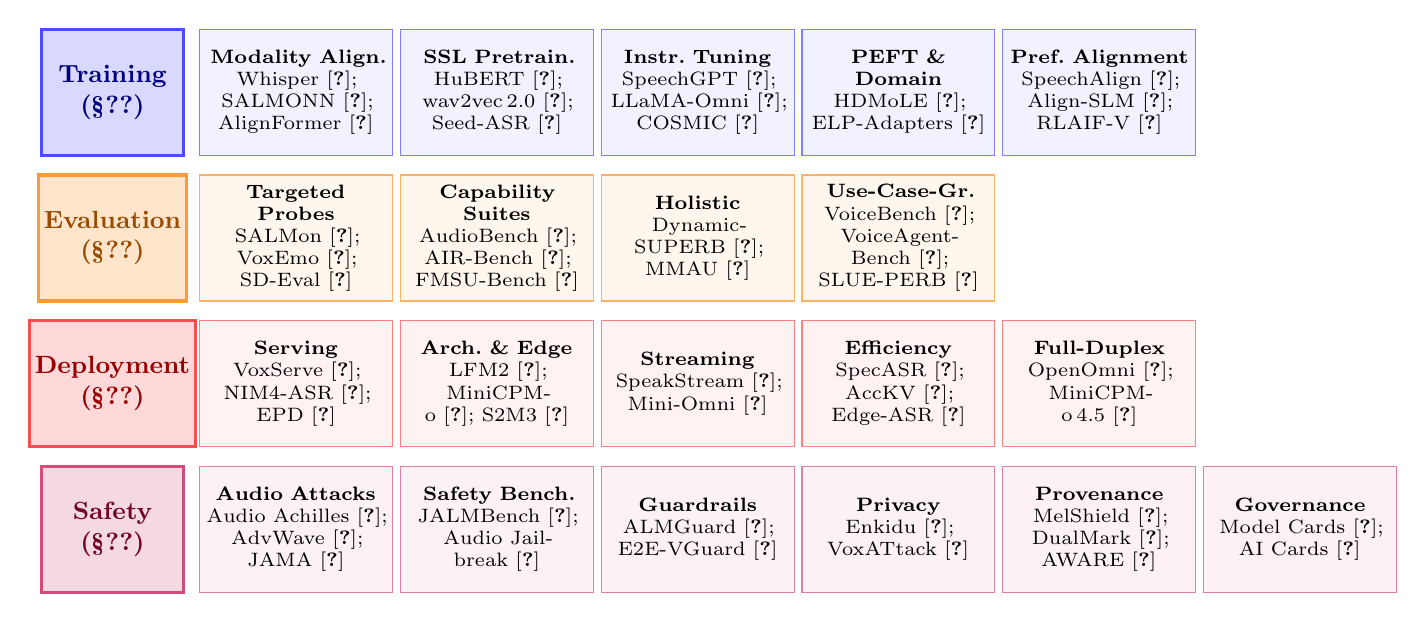
\begin{tikzpicture}[
  every node/.style={align=center, inner sep=2pt},
  stageT/.style={rectangle, draw=blue!70, very thick, fill=blue!15,
                 minimum width=1.8cm, minimum height=1.6cm,
                 font=\small\bfseries\color{blue!50!black}, align=center},
  stageE/.style={rectangle, draw=orange!80, very thick, fill=orange!20,
                 minimum width=1.8cm, minimum height=1.6cm,
                 font=\small\bfseries\color{orange!60!black}, align=center},
  stageD/.style={rectangle, draw=red!70, very thick, fill=red!15,
                 minimum width=1.8cm, minimum height=1.6cm,
                 font=\small\bfseries\color{red!60!black}, align=center},
  stageS/.style={rectangle, draw=purple!70, very thick, fill=purple!15,
                 minimum width=1.8cm, minimum height=1.6cm,
                 font=\small\bfseries\color{purple!60!black}, align=center},
  topicT/.style={rectangle, draw=blue!50, thin, fill=blue!5,
                 minimum width=2.45cm, minimum height=1.6cm,
                 text width=2.25cm, font=\scriptsize, anchor=west, align=center},
  topicE/.style={rectangle, draw=orange!60, thin, fill=orange!7,
                 minimum width=2.45cm, minimum height=1.6cm,
                 text width=2.25cm, font=\scriptsize, anchor=west, align=center},
  topicD/.style={rectangle, draw=red!50, thin, fill=red!5,
                 minimum width=2.45cm, minimum height=1.6cm,
                 text width=2.25cm, font=\scriptsize, anchor=west, align=center},
  topicS/.style={rectangle, draw=purple!50, thin, fill=purple!5,
                 minimum width=2.45cm, minimum height=1.6cm,
                 text width=2.25cm, font=\scriptsize, anchor=west, align=center}
]
% ROW 1: TRAINING
\node[stageT] (s1) at (0,0) {Training\\(\S\ref{sec:training_strategies})};
\node[topicT] (t1a) at (1.1,0)  {\textbf{Modality Align.}\\ Whisper~\cite{radford2023robust}; SALMONN~\cite{tang2023salmonn}; AlignFormer~\cite{fan2025alignformer}};
\node[topicT] (t1b) at (3.65,0) {\textbf{SSL Pretrain.}\\ HuBERT~\cite{hsu2021hubert}; wav2vec\,2.0~\cite{baevski2020wav2vec}; Seed-ASR~\cite{bai2024seed}};
\node[topicT] (t1c) at (6.20,0) {\textbf{Instr.~Tuning}\\ SpeechGPT~\cite{zhang2023speechgptempoweringlargelanguage}; LLaMA-Omni~\cite{fang2025llamaomniseamlessspeechinteraction}; COSMIC~\cite{pan2024cosmicdataefficientinstructiontuning}};
\node[topicT] (t1d) at (8.75,0) {\textbf{PEFT \& Domain}\\ HDMoLE~\cite{mu2025hdmolemixtureloraexperts}; ELP-Adapters~\cite{inoue2024elpadaptersparameterefficientadapter}};
\node[topicT] (t1e) at (11.30,0){\textbf{Pref.~Alignment}\\ SpeechAlign~\cite{zhang2024speechalignaligningspeechgeneration}; Align-SLM~\cite{lin2025alignslmtextlessspokenlanguage}; RLAIF-V~\cite{yu2024rlaifvopensourceaifeedback}};

% ROW 2: EVALUATION
\node[stageE] (s2) at (0,-1.85) {Evaluation\\(\S\ref{sec:evaluation_benchmarking})};
\node[topicE] at (1.1,-1.85)  {\textbf{Targeted Probes}\\ SALMon~\cite{maimon2024salmon}; VoxEmo~\cite{zhang2026voxemo}; SD-Eval~\cite{ao2024sdeval}};
\node[topicE] at (3.65,-1.85) {\textbf{Capability Suites}\\ AudioBench~\cite{wang2025audiobench}; AIR-Bench~\cite{yang2024airbench}; FMSU-Bench~\cite{li2026fmsubench}};
\node[topicE] at (6.20,-1.85) {\textbf{Holistic}\\ Dynamic-SUPERB~\cite{huang2024dynamicsuperb}; MMAU~\cite{sakshi2024mmau}};
\node[topicE] at (8.75,-1.85) {\textbf{Use-Case-Gr.}\\ VoiceBench~\cite{chen2024voicebench}; VoiceAgentBench~\cite{jain2025voiceagentbench}; SLUE-PERB~\cite{shon2023slue}};

% ROW 3: DEPLOYMENT
\node[stageD] (s3) at (0,-3.7) {Deployment\\(\S\ref{sec:deployment})};
\node[topicD] at (1.1,-3.7)  {\textbf{Serving}\\ VoxServe~\cite{kamahori2026voxserve}; NIM4-ASR~\cite{xie2026nim4asr}; EPD~\cite{singh2025epd}};
\node[topicD] at (3.65,-3.7) {\textbf{Arch.~\& Edge}\\ LFM2~\cite{amini2025lfm2}; MiniCPM-o~\cite{cui2026minicpmo}; S2M3~\cite{yoon2025s2m3}};
\node[topicD] at (6.20,-3.7) {\textbf{Streaming}\\ SpeakStream~\cite{bai2025speakstream}; Mini-Omni~\cite{xie2024miniomni}};
\node[topicD] at (8.75,-3.7) {\textbf{Efficiency}\\ SpecASR~\cite{wei2025specasr}; AccKV~\cite{jiang2025acckv}; Edge-ASR~\cite{feng2025edgeasr}};
\node[topicD] at (11.30,-3.7){\textbf{Full-Duplex}\\ OpenOmni~\cite{luo2025openomni}; MiniCPM-o\,4.5~\cite{cui2026minicpmo}};

% ROW 4: SAFETY
\node[stageS] (s4) at (0,-5.55) {Safety\\(\S\ref{sec:safety_privacy_governance})};
\node[topicS] at (1.1,-5.55)  {\textbf{Audio Attacks}\\ Audio Achilles~\cite{yang2024audioachillesheelred}; AdvWave~\cite{kang2024advwavestealthyadversarialjailbreak}; JAMA~\cite{krishnan2026optimizingmultimodaljailbreaksspoken}};
\node[topicS] at (3.65,-5.55) {\textbf{Safety Bench.}\\ JALMBench~\cite{peng2026jalmbenchbenchmarkingjailbreakvulnerabilities}; Audio Jailbreak~\cite{song2025audiojailbreakopencomprehensive}};
\node[topicS] at (6.20,-5.55) {\textbf{Guardrails}\\ ALMGuard~\cite{jin2025almguardsafetyshortcutsguardrails}; E2E-VGuard~\cite{zhang2025e2evguardadversarialpreventionproduction}};
\node[topicS] at (8.75,-5.55) {\textbf{Privacy}\\ Enkidu~\cite{feng2025enkiduuniversalfrequentialperturbation}; VoxATtack~\cite{aloradi2026voxattackmultimodalattackvoice}};
\node[topicS] at (11.30,-5.55){\textbf{Provenance}\\ MelShield~\cite{jin2026melshieldrobustmeldomainaudio}; DualMark~\cite{yang2025dualmarkidentifyingmodeltraining}; AWARE~\cite{pavlović2026awareaudiowatermarkingadversarial}};
\node[topicS] at (13.85,-5.55){\textbf{Governance}\\ Model Cards~\cite{Mitchell_2019}; AI Cards~\cite{golpayegani2024aicardsappliedframework}};
\end{tikzpicture}
\caption{Paper taxonomy of Speech LLM lifecycle research covered by
this survey. Representative methods and systems are grouped under the
four lifecycle stages introduced in
Figure~\ref{fig:lifecycle}. The taxonomy lists 2--3 representative
works per sub-topic to indicate scope; the full reference list and
benchmark coding are released as supplementary material.}
\label{fig:taxonomy}
\end{figure*}


Section~\ref{sec:background} introduces the speech-specific concepts
the survey relies on. Section~\ref{sec:training_strategies}
consolidates training strategies. Sections
\ref{sec:evaluation_benchmarking}, \ref{sec:deployment}, and
\ref{sec:safety_privacy_governance} develop the lifecycle audit for
evaluation, deployment, and safety. We close with open challenges
(Section~\ref{sec:future_directions}) and a synthesis
(Section~\ref{sec:conclusion}). The lifecycle map in
Figure~\ref{fig:lifecycle} traces these stages and the couplings the
survey emphasizes.

\begin{figure}[!t]
\centering
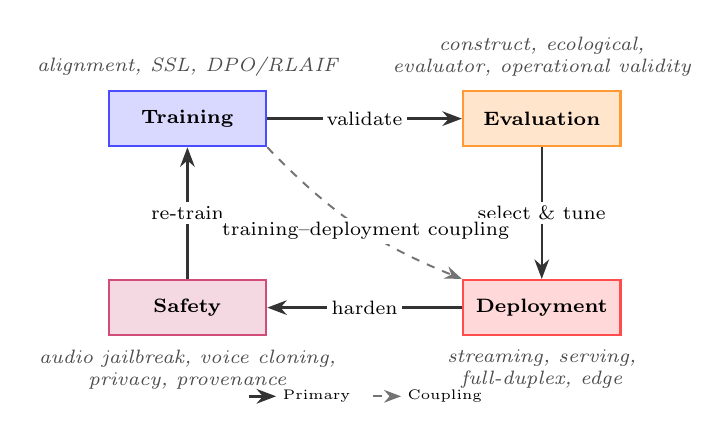
\begin{tikzpicture}[
  >=Stealth,
  every node/.style={font=\scriptsize},
  stage/.style={
    rectangle, draw=black!75, thick,
    minimum width=2.0cm, minimum height=0.7cm,
    align=center, fill=black!5
  },
  artifact/.style={font=\scriptsize\itshape, text=black!70, align=center},
  primary/.style={->, line width=0.9pt, draw=black!80},
  coupling/.style={->, line width=0.7pt, draw=black!55, dashed},
  arrowlabel/.style={font=\scriptsize, fill=white, inner sep=1.5pt}
]
% Four lifecycle stages at corners of a 4.5cm x 2.4cm rectangle (single-column fit).
\node[stage, fill=blue!15,   draw=blue!70]   (train)  at (0,2.4)  {\textbf{Training}};
\node[stage, fill=orange!20, draw=orange!80] (eval)   at (4.5,2.4){\textbf{Evaluation}};
\node[stage, fill=red!15,    draw=red!70]    (deploy) at (4.5,0)  {\textbf{Deployment}};
\node[stage, fill=purple!15, draw=purple!70] (safety) at (0,0)    {\textbf{Safety}};

% Artifacts placed OUTSIDE the wheel so they do not crowd the
% re-train / select-and-tune arrows in the interior.
\node[artifact, above=0.05cm of train]  {alignment, SSL, DPO/RLAIF};
\node[artifact, above=0.05cm of eval]   {construct, ecological,\\evaluator, operational validity};
\node[artifact, below=0.05cm of deploy] {streaming, serving,\\full-duplex, edge};
\node[artifact, below=0.05cm of safety] {audio jailbreak, voice cloning,\\privacy, provenance};

% Primary lifecycle arrows (clockwise) along the outside of the rectangle
\draw[primary] (train)  -- node[arrowlabel, midway] {validate}      (eval);
\draw[primary] (eval)   -- node[arrowlabel, midway] {select \& tune} (deploy);
\draw[primary] (deploy) -- node[arrowlabel, midway] {harden}        (safety);
\draw[primary] (safety) -- node[arrowlabel, midway] {re-train}      (train);

% One diagonal cross-stage coupling, bent slightly to avoid arrow labels
\draw[coupling] (train.south east) to[bend right=12]
  node[arrowlabel, pos=0.55] {training--deployment coupling}
  (deploy.north west);

% Legend as a single horizontal row below the wheel
\node[anchor=north, font=\tiny] at (2.25,-0.9) {
  \begin{tabular}{@{}c@{\hspace{2pt}}l@{\hspace{8pt}}c@{\hspace{2pt}}l@{}}
    \tikz[baseline=-0.6ex] \draw[primary] (0,0) -- (0.35,0); & Primary &
    \tikz[baseline=-0.6ex] \draw[coupling] (0,0) -- (0.35,0); & Coupling \\
  \end{tabular}
};
\end{tikzpicture}
\caption{The Speech LLM lifecycle as a coupled system. Solid arrows
trace the conventional cycle from training through evaluation,
deployment, and safety, with re-training closing the loop. The dashed
diagonal highlights the survey's central claim that the cycle is not
purely sequential: training choices shape deployment feasibility,
and the consequences of evaluation, deployment, and safety choices
feed back through re-training.}
\label{fig:lifecycle}
\end{figure}

To make the cross-stage couplings concrete, Table~\ref{tab:coupling_evidence}
records five examples where a training, evaluation, or deployment choice
documented in the literature produced a visible consequence in a
downstream stage.

\begin{table*}[t]
\caption{Concrete cross-stage couplings observed in the literature
covered by this survey. Each row links a specific upstream decision to
a documented downstream consequence, illustrating that the four
lifecycle stages are not independent.}
\label{tab:coupling_evidence}
\centering
\footnotesize
\begin{tabularx}{\textwidth}{|p{0.13\textwidth}|X|X|X|}
\hline
\textbf{Upstream stage} & \textbf{Decision / observation} &
\textbf{Downstream stage affected} & \textbf{Documented consequence} \\
\hline
Training &
Whisper-style weakly supervised pretraining emphasizes transcription
quality \cite{radford2023robust}. &
Evaluation &
Benchmarks inherit ASR-centric metrics; paralinguistic and prosodic
validity are under-measured (Section~\ref{subsec:eval_coverage}). \\
\hline
Training &
Adapter / Q-Former bridge between speech encoder and language model
\cite{tang2023salmonn,fan2025alignformer}. &
Deployment &
Bridge layer adds latency; full-duplex stacks must redesign streaming
boundary (Section~\ref{sec:deployment}). \\
\hline
Evaluation &
Multilinguality coverage is fragmented across incompatible metrics
\cite{liu2025seallmsaudio,papi2025hearing2translate}. &
Deployment &
Practitioners cannot rank multilingual systems for production without
re-running on a target language slice (Section~\ref{sec:deployment}). \\
\hline
Evaluation &
LLM-as-judge protocols underlie open-ended scoring with only moderate
human correlation \cite{ao2024sdeval,zheng2023judging}. &
Safety &
Judge-based reward signals can miss unsafe prosody or jailbreaks
triggered by acoustic content (Section~\ref{sec:safety_privacy_governance}). \\
\hline
Deployment &
Quantization and KV-cache pruning are applied for edge feasibility
\cite{xie2024miniomni}. &
Safety &
Downstream safety classifiers and watermark detectors can degrade
under aggressive compression
(Section~\ref{sec:safety_privacy_governance}). \\
\hline
\end{tabularx}
\end{table*}
\FloatBarrier
\section{Background: Speech LLMs and Their Lifecycle Challenges}
\label{sec:background}

We assume reader familiarity with the Transformer-based language model
backbone (e.g., \citep{vaswani2017attention,radford2019language,brown2020language})
and standard supervised, instruction-tuned, and RLHF-aligned text LLM
pipelines. This section sets up the speech-specific concepts the rest of
the survey relies on.

\paragraph{Speech LLMs.}
We use \emph{Speech LLM} to refer to an LLM-based system that consumes,
reasons over, or generates speech as part of language interaction. This
includes speech-to-text recognition coupled with an LLM (cascaded),
speech-to-text and speech-to-speech models that share a single backbone
(end-to-end), and omni-modal models that integrate speech with text and
other modalities \citep{cui2024recent,peng2025surveyspeechlargelanguage}.

\paragraph{Why speech is different.}
Three properties of speech shape every lifecycle stage of Speech LLMs.
First, speech is a continuous, high-dimensional, multi-channel signal that
carries linguistic content, paralinguistics, speaker identity, scene
context, and timing simultaneously. Second, parallel speech-text data is
expensive and unevenly distributed across languages and domains, so most
training pipelines depend on weak supervision or self-supervision
\citep{radford2023robust,hsu2021hubert}. Third, speech interaction is
inherently real-time: a model that produces a correct transcript or
response too late may fail the interaction even if its content is
accurate. Together, these properties drive the design choices reviewed in
the following sections.

\paragraph{Lifecycle framing.}
The remainder of the survey is organized around four lifecycle stages:
training strategies (Section~\ref{sec:training_strategies}), evaluation
and benchmarking (Section~\ref{sec:evaluation_benchmarking}), deployment
and real-time interaction (Section~\ref{sec:deployment}), and safety,
privacy, and governance (Section~\ref{sec:safety_privacy_governance}).
The four stages are tightly coupled. Training choices determine what
benchmarks reveal; benchmarks reveal what deployment must defend
against; deployment constraints reshape which training and evaluation
trade-offs are acceptable; and safety risks span all three.

\section{Training Strategies for Speech LLMs}
\label{sec:training_strategies}

Building Speech LLMs requires extending the text-LLM training pipeline to
account for the continuous, multi-channel nature of speech. We organize
the literature around four training stages: (i) modality alignment and
pretraining, (ii) fine-tuning and adaptation, (iii) preference alignment,
and (iv) cross-cutting design issues that connect training to the
remainder of the lifecycle. Throughout, we emphasize choices that have
downstream implications for evaluation
(Section~\ref{sec:evaluation_benchmarking}), deployment
(Section~\ref{sec:deployment}), and safety
(Section~\ref{sec:safety_privacy_governance}).

\subsection{Modality Alignment and Pretraining}
\label{subsec:training_pretraining}

Speech and text differ in two ways that complicate joint modeling: speech
sequences are typically much longer than their text counterparts, and
speech embeddings live in a separate representation space from text
embeddings \citep{fan2025alignformer,bai2024seed}. Modality alignment
modules and acoustic pretraining strategies address these mismatches.

\paragraph{Alignment modules.}
Modular Speech LLMs combine a pretrained speech encoder (e.g., Whisper
\citep{radford2023robust}, HuBERT \citep{hsu2021hubert}, wav2vec~2.0
\citep{baevski2020wav2vec}) with a partly frozen text LLM through a
trainable bridge. \emph{AlignFormer} \citep{fan2025alignformer} pairs a
Connectionist Temporal Classification (CTC) layer with a Q-Former-style
attention module to map variable-length acoustic features to discrete
text-aligned tokens. \emph{Seed-ASR Converter} \citep{bai2024seed} learns
a context-aware transformation that improves multilingual generalization.
\emph{SALMONN}'s Q-Former \citep{tang2023salmonn} and the OSUM adapter
\citep{geng2025osum} use a small set of trainable queries to distill
semantically rich acoustic representations into the LLM's input space.
As an alternative to adapter-based bridging, X-OPD
\citep{cao2026xopd} distills text-LLM capabilities into a speech-LLM via
cross-modal on-policy rollouts, bypassing the need for paired
speech-text supervision altogether. Empirical alignment quality can be
probed via the Automatic Latent Alignment Score (ALAS)
\citep{mousavi2025alas}, which uses Whisper timestamps as a reference and
reports that deeper transformer layers align better for semantic tasks
while earlier layers align better for paralinguistic tasks.

\paragraph{Self-supervised pretraining.}
Speech LLMs adapt the masked-prediction and clustering objectives from
text SSL to raw audio. Representative methods include UniSpeech-SAT
\citep{chen2022unispeech}, which adds speaker-aware objectives to the SSL
loss; DinoSR \citep{liu2023dinosr}, which combines self-distillation with
masked acoustic modeling; and Seed-ASR \citep{bai2024seed}, which scales a
BERT-style masked-prediction pretraining to millions of hours of speech
to produce the LUISE encoder, subsequently aligned to a language model.

\paragraph{Joint and weakly supervised pretraining.}
Two further pretraining paradigms reduce reliance on parallel speech-text
data. \emph{Cold-start joint modeling} initializes both speech and
language components together, as in Generative Spoken Language Modeling
(GSLM) \citep{lakhotia2021generative} and SPIRIT-LM \citep{nguyen2025spirit},
yielding tighter cross-modal interactions than methods that freeze the
language model. \emph{Weakly supervised pretraining at scale}, exemplified
by Whisper \citep{radford2023robust}'s 680{,}000-hour multilingual corpus,
trades exact transcription quality for breadth and produces strong
zero-shot transcription, translation, and detection capabilities. Many
later systems (OSUM \citep{geng2025osum}, SALMONN \citep{tang2023salmonn})
build directly on Whisper-style encoders, treating large-scale weak
supervision as the de facto foundation.

\subsection{Fine-Tuning and Adaptation}
\label{subsec:training_finetuning}

Pretraining yields foundations; fine-tuning produces task-aligned
behavior. Speech LLM fine-tuning takes three main forms.

\paragraph{Instruction tuning.}
Instruction tuning aligns Speech LLMs to user intent in spoken dialogue,
question answering, and editing tasks. SpeechGPT
\citep{zhang2023speechgptempoweringlargelanguage} integrates discrete
speech tokens into a decoder-only LLM backbone with strong zero-shot
generalization. COSMIC \citep{pan2024cosmicdataefficientinstructiontuning}
trains a Q-Former bridge on 450 hours of speech plus GPT-3.5-generated
QA pairs, achieving competitive ASR and speech-to-text translation with
limited paired data. InstructSpeech \citep{huang2024instructspeech} uses
hierarchical adapters and multi-step reasoning for fine-grained semantic
and acoustic editing. LLaMA-Omni
\citep{fang2025llamaomniseamlessspeechinteraction} pairs a frozen Whisper
encoder with LLaMA-3.1-8B-Instruct and a streaming decoder, reporting
226\,ms response latency without intermediate transcription. More
recently, Audio-FLAN \citep{xue2025audioflan} demonstrates that scaling
instruction data to over 100 million instances across 80 audio tasks
yields substantial gains, signaling a shift toward
massive-scale instruction tuning.

\paragraph{Parameter-efficient tuning.}
Parameter-efficient fine-tuning (PEFT) updates a small fraction of model
parameters while freezing the rest, reducing compute cost and mitigating
catastrophic forgetting. HDMoLE \citep{mu2025hdmolemixtureloraexperts}
combines hierarchical LoRA adapters with mixture-of-experts routing for
joint accent and domain adaptation, updating $\sim$9.6\% of parameters
while matching full fine-tuning. ELP-Adapters
\citep{inoue2024elpadaptersparameterefficientadapter} insert lightweight
modules at multiple abstraction levels of pretrained encoders such as
WavLM, enabling targeted adaptation with minimal parameter footprint.
Zipper-LoRA \citep{mei2026zipperlora} further advances speech-specific
PEFT by introducing language-conditioned routing with rank-level
decoupling for multilingual speech recognition.

\paragraph{Domain-specific tuning.}
Specialized domains (medical, financial, technical) often have
constrained paired speech-text resources. Low-resource adaptation via
unpaired domain-specific text \citep{fang2025lowresourcedomainadaptationspeech}
fine-tunes the language decoder with LoRA while preserving alignment via
real-time evaluation, reducing domain WER without harming general
performance. Decoder-only context perturbation \citep{suh2024improving}
freezes the encoder and randomizes domain descriptions during decoder
fine-tuning to mitigate overfitting and forgetting, with successful
applications to earnings calls and medical dialogue.

\subsection{Post-Training Preference Alignment}
\label{subsec:training_alignment}

Pretraining and fine-tuning equip Speech LLMs with capability; preference
alignment shapes their behavior to match user expectations for
helpfulness, safety, and naturalness. This is especially consequential in
speech, where prosody, pacing, and emotion strongly influence perceived
quality \citep{communication2023seamlessmultilingualexpressivestreaming}.

\paragraph{Reinforcement Learning from Human Feedback (RLHF).}
RLHF \citep{ouyang2022training,christiano2017deep} trains a reward model
on human-labeled preference pairs and then optimizes the base model
against it. The reward model uses a pairwise ranking loss that converts
human comparisons into a scalar reward:
\begin{equation}
\mathcal{L}^{\text{reward}}(\phi) = -\log \sigma\left( r_\phi(x, y_1) - r_\phi(x, y_2) \right),
\end{equation}
where $x$ is the prompt, $y_1$ is preferred over $y_2$, and $r_\phi$
scores responses. The base model is then optimized via policy-gradient
methods (typically PPO \citep{schulman2017proximalpolicyoptimizationalgorithms}
in text settings) with a KL constraint to a reference model. RLHF is
expensive in human annotation and unstable to tune, particularly in
speech, where preference data must capture acoustic and paralinguistic
quality in addition to content. As a result, Speech LLMs typically
substitute RLHF with lighter alternatives \citep{rafailov2023direct}.

\paragraph{Direct Preference Optimization (DPO).}
DPO \citep{rafailov2023direct} eliminates the explicit reward model by
expressing the preference loss directly in terms of the policy:
\begin{equation}
\mathcal{L}_{\mathrm{DPO}}(\theta)
= - \mathbb{E}_{x,y_w,y_l}
\left[
\log \sigma \left(
\beta \left(
\log \frac{\pi_\theta(y_w \mid x)}{\pi_{\mathrm{ref}}(y_w \mid x)}
-
\log \frac{\pi_\theta(y_l \mid x)}{\pi_{\mathrm{ref}}(y_l \mid x)}
\right)
\right)
\right].
\end{equation}

DPO matches or exceeds RLHF on text alignment tasks while using a single
training stage. Speech LLMs have rapidly adopted it. SpeechAlign
\citep{zhang2024speechalignaligningspeechgeneration} iteratively refines a
zero-shot TTS model on LibriSpeech and VCTK, surpassing RLHF-PPO on Word
Error Rate, Speaker Similarity, and human ratings. Align-SLM
\citep{lin2025alignslmtextlessspokenlanguage} extends DPO to a textless
spoken language model trained on LibriSpeech and Multilingual LibriSpeech,
outperforming Moshi and SPIRIT-LM on the spoken StoryCloze benchmark.
OpenOmni \citep{luo2025openomniadvancingopensourceomnimodal} introduces a
Connectionist Temporal Classification variant of DPO (CTC-DPO) for
emotionally coherent speech generation, reporting strong results on the
EO2S-9k bilingual emotional speech benchmark. Beyond pairwise
comparisons, Emo-LiPO \citep{lin2026emolipo} proposes listwise preference
optimization for speech emotion intensity, suggesting that richer
ranking signals can further improve alignment quality.

\paragraph{Reinforcement Learning from AI Feedback (RLAIF).}
RLAIF \citep{lee2024rlaifvsrlhfscaling,bai2022constitutionalaiharmlessnessai}
replaces human preference annotation with AI-generated labels, trading a
small accuracy cost for substantially improved scalability. Lee et al.\
show that direct RLAIF (d-RLAIF) prompts an AI labeler at training time
and matches or exceeds RLHF on summarization and dialogue. RLAIF-V
\citep{yu2024rlaifvopensourceaifeedback} extends this to multimodal models
with deconfounded generation and atomic claim decomposition; the 12B
variant reduces its overall hallucination rate by 32.4\% through
self-alignment, surpassing GPT-4V in trustworthiness. In speech,
AlignSLM \citep{lin2025alignslmtextlessspokenlanguage} uses semantic
metrics on AI-generated speech continuations to construct preference data
for DPO, achieving state-of-the-art results on spoken StoryCloze.

\paragraph{Comparison.}
Table~\ref{tab:alignment_comparison} compares RLHF, DPO, and RLAIF
alongside their speech-specific evaluation considerations. The choice
depends not only on annotation cost, but also on what evaluation regime
(Section~\ref{sec:evaluation_benchmarking}) is available: methods that
require dense per-turn or per-utterance ratings are difficult when
benchmarks can only score complete responses.

\begin{table*}[t]
\caption{Comparison of preference alignment methods for Speech LLMs. The
last column links each method to evaluation considerations developed in
Section~\ref{sec:evaluation_benchmarking}.}
\label{tab:alignment_comparison}
\centering
\scriptsize
\begin{tabularx}{\linewidth}{lXXXX}
\toprule
\textbf{Aspect} & \textbf{RLHF} & \textbf{DPO} & \textbf{RLAIF} & \textbf{Speech-evaluation hook} \\
\midrule
\textbf{Annotation source} & Human preference pairs & Human preference pairs; some implementations mix synthetic data & AI-generated preference pairs & Speech requires acoustic + paralinguistic judgements; LLM judges are still moderate-correlation \citep{zheng2023judging} \\
\midrule
\textbf{Optimization} & Policy gradient (e.g., PPO) & Direct preference loss & Reward learning or DPO-style & Construct/evaluator validity (Section~\ref{sec:evaluation_benchmarking}) determines which optimization signal is reliable \\
\midrule
\textbf{Reward model} & Required & Not required & Required (or implicit) & A reward trained on transcripts misses acoustic quality; speech reward models remain underdeveloped \\
\midrule
\textbf{Engineering overhead} & High (multi-stage pipeline) & Moderate (single-stage) & Moderate (auto-labeling pipeline) & Operational validity hooks: alignment cost shapes deployment cycle (Section~\ref{sec:deployment}) \\
\midrule
\textbf{Speech adoption} & Limited (manual effort, slow iteration) & Promising: SpeechAlign, Align-SLM, OpenOmni & Emerging: RLAIF-V, AlignSLM & Adoption tracks the availability of speech-aware judges and benchmarks \\
\midrule
\textbf{Scalability} & Limited by annotation cost & Improved efficiency & High (AI-supervised) & Scaling depends on whether evaluation can detect over-optimization (Section~\ref{sec:evaluation_benchmarking}) \\
\bottomrule
\end{tabularx}
\end{table*}

\subsection{Cross-Cutting Training Issues}
\label{subsec:training_crosscutting}

Three training-design decisions have outsized influence on the rest of
the lifecycle and motivate later sections.

\emph{Data sufficiency.} Self-supervised and weakly supervised
pretraining on tens to hundreds of thousands of hours has become the
default \citep{radford2023robust,bai2024seed}, but parallel speech-text
data remains scarce for low-resource languages, scripts, and domains.
This data imbalance reappears in evaluation: most multilingual
benchmarks under-sample non-Latin scripts (Section~\ref{sec:evaluation_benchmarking}).

\emph{Alignment quality.} Whether alignment modules preserve
paralinguistic content varies substantially across architectures
\citep{mousavi2025alas,fan2025alignformer}. Benchmarks such as SALMon and
FMSU-Bench show that semantically capable Speech LLMs frequently fail at
acoustic-semantic binding (Section~\ref{sec:evaluation_benchmarking}),
which suggests that alignment quality, not language modeling, is often
the bottleneck.

\emph{Deployment-aware training.} Few training pipelines optimize
explicitly for streaming, latency, or interruption handling. Models
designed for offline benchmarks may compute correctly but respond too
late for natural interaction, motivating the architecture and protocol
choices analyzed in Section~\ref{sec:deployment}. Safety-aware training
is similarly under-developed: text safety alignment does not
automatically transfer to audio inputs, as
Section~\ref{sec:safety_privacy_governance} demonstrates.

These cross-cutting issues connect the training section to the rest of the survey. The following sections examine whether current evaluation, deployment, and safety practices can measure the limitations introduced by training choices.

\section{Evaluation and Benchmarking}
\label{sec:evaluation_benchmarking}

This section is a meta-evaluation of Speech LLM benchmarks rather than a
catalog. We ask three questions: what current benchmarks measure, how
reliably they measure it, and what remains invisible to them. Building on
text-LLM evaluation efforts such as HELM, MMLU, and BIG-Bench
\cite{liang2022helm,hendrycks2021measuring,srivastava2023beyond}, we identify
the speech-specific extensions that an IPM-quality survey must demand.

\subsection{From LLM Evaluation to Speech LLM Evaluation}
\label{subsec:eval_setup}

Evaluation is where claims about Speech LLM training become claims about
capability, reliability, and deployability. Classical machine learning
organizes evaluation around three elements: a dataset, a protocol, and a
metric. LLM evaluation complicates all three. Open-ended generation weakens
single-label scoring \cite{liang2022helm}, prompt and decoding choices
introduce non-trivial score variance \cite{hendrycks2021measuring},
training-data contamination is difficult to rule out
\cite{srivastava2023beyond}, and LLM-as-judge protocols create a circular
dependency in which the evaluator itself becomes an object of evaluation
\cite{zheng2023judging}.

Speech adds another layer of difficulty. A speech input is not a text
sequence but a \emph{multi-channel acoustic signal} carrying linguistic
content, paralinguistic information, speaker traits, accent, acoustic
scene, timing, and interaction dynamics simultaneously. Word error rate,
BLEU, exact match, and MOS-style scores are therefore necessary but
incomplete: each observes only a slice of speech behavior. A system can
transcribe words correctly while missing emotion, produce a semantically
plausible answer while ignoring background events, or generate a correct
response too late for natural conversation. Recent benchmarks expose these
failures from different angles:

\begin{itemize}
  \item \textbf{Acoustic--semantic misalignment}: SALMon \cite{maimon2024salmon} probes whether models bind acoustic context to spoken content.
  \item \textbf{Fine-grained paralinguistic blindness}: FMSU-Bench \cite{li2026fmsubench} and VoxEmo \cite{zhang2026voxemo} expose weaknesses in micro-acoustic perception.
  \item \textbf{Multilingual and code-switching fragility}: Dynamic-SUPERB \cite{huang2024dynamicsuperb} and SCENEBench \cite{iyer2026scenebench} include explicit cross-lingual stress cases.
  \item \textbf{Interaction instability}: StyleBench \cite{zhao2026stylebench} and VoiceAgentBench \cite{jain2025voiceagentbench} target multi-turn behavior and tool use.
  \item \textbf{Cross-modal safety divergence}: VoiceBench \cite{chen2024voicebench} shows that safety responses can change between text and speech modes; we develop this further in Section~\ref{sec:safety_privacy_governance}.
\end{itemize}

The question for evaluation is therefore not only whether a model performs
well on a task, but whether the benchmark measures the speech-specific
behavior that matters for real use. Subsequent subsections audit whether
current benchmarks meet that bar.

\subsection{Benchmark Corpus and Scope}
\label{subsec:eval_corpus}

We analyze 18 benchmarks from 2024--2026 that evaluate speech-relevant
capabilities of LLM-based systems. The pool includes benchmarks designed
directly for Speech LLMs, broader Audio LLM benchmarks when their tasks
transfer to speech interaction (judged by whether at least half their
prompts contain spoken language as primary signal), and voice-assistant,
agentic, multilingual, paralinguistic, and auditory-knowledge benchmarks
when they evaluate speech-relevant behavior. Traditional ASR and TTS
benchmarks are used only as background unless embedded in a Speech LLM
evaluation protocol. Of the 18 benchmarks, 3 are peer-reviewed
(SD-Eval at the NeurIPS 2024 Datasets and Benchmarks track \cite{ao2024sdeval}, Dynamic-SUPERB at ICLR 2025
\cite{huang2024dynamicsuperb},
SLUE-PERB at INTERSPEECH 2023 \cite{shon2023slue}); the remaining 15 are
arXiv preprints as of June 2026 (we count only benchmarks with confirmed
proceedings or journal publication, not papers under review). We label
preprint evidence as such throughout and avoid claims that depend on
un-peer-reviewed sample sizes or rankings.

For Figure~\ref{fig:benchmark_heatmap}, we coded capability coverage as
a binary indicator: a dimension is counted when the benchmark
explicitly defines a task, supplies test data, and reports a metric for
that dimension; partial or implicit coverage was not counted.
Disagreements during coding were resolved by re-reading the original
paper rather than by inference.

\paragraph{Search and selection.}
Benchmarks were identified via Google Scholar, the arXiv
\texttt{cs.CL} and \texttt{eess.AS} categories, the ACL Anthology, and
the proceedings of NeurIPS, ICLR, ICML, INTERSPEECH, and ICASSP,
covering January 2024 through June 2026. We searched for
``Speech LLM'', ``Audio LLM'', ``voice assistant benchmark'', ``speech
evaluation'', ``audio jailbreak'', ``full-duplex speech'', and
``streaming speech model''. A benchmark was included when it evaluated
an LLM-based system on speech or audio input, defined tasks with test
data and metrics, and covered at least one capability dimension from
Figure~\ref{fig:benchmark_heatmap}; pure ASR or TTS benchmarks were
excluded unless they were embedded in a Speech LLM evaluation protocol.
Coding for Figure~\ref{fig:benchmark_heatmap} was performed by a single
reviewer with disagreements resolved by re-reading the source paper
rather than by inference; per-benchmark reading notes are released as
supplementary material so that the coding can be independently
validated by the community. We label this corpus as a 2024--2026
snapshot; given that fifteen of the eighteen benchmarks were arXiv
preprints at the time of writing, some entries may have been
peer-reviewed or superseded by the time of publication, and the
analysis should be read as a contemporaneous audit rather than a final
record.

\subsection{A Two-Axis Taxonomy of Speech LLM Benchmarks}
\label{subsec:eval_taxonomy}

A single-axis taxonomy by task family is useful but insufficient. The same
benchmark can be broad in modality coverage, narrow in evaluation lens, and
partially anchored to a deployment use case. We organize the benchmark
landscape using two orthogonal axes. The \emph{scope} axis describes
breadth and depth: targeted probe, capability-focused suite, holistic
suite, or use-case-grounded evaluation. The \emph{lens} axis describes the
benchmark's dominant evaluative perspective: capability, use case,
phenomenon, or knowledge. Table~\ref{tab:benchmark_taxonomy} shows primary
placements with secondary lenses noted in footnotes; placements are not
exclusive. VoiceBench is use-case-grounded but also probes robustness and
safety; SCENEBench is primarily phenomenon-oriented but has use-case
flavor; FMSU-Bench can be read as both capability-focused and a targeted
paralinguistic probe.

We read Table~\ref{tab:benchmark_taxonomy} by row first (scope) and then by
column (lens). Cells with multiple entries indicate saturation of
attention; empty cells indicate evaluation blind spots.
\begin{table}[t]
\centering
\caption{Primary placement of 18 Speech LLM benchmarks (2024--2026) under a
scope $\times$ lens taxonomy.}
\label{tab:benchmark_taxonomy}
\scriptsize
\setlength{\tabcolsep}{4pt}
\renewcommand{\arraystretch}{1.18}

\begin{threeparttable}
\begin{tabularx}{\textwidth}{
  >{\RaggedRight\arraybackslash\bfseries}p{0.13\textwidth}
  Y Y Y Y
}
\toprule
Scope / Lens & Capability & Use case & Phenomenon & Knowledge \\
\midrule

Targeted probe
&
SALMon (8 tasks)\cite{maimon2024salmon};
VoxEmo (35 corpora)\cite{zhang2026voxemo};
StyleBench (4 dims)\cite{zhao2026stylebench};
SD-Eval\tnote{$\dagger$} (4 dims, 7.3K)\cite{ao2024sdeval}
&
\na
&
LoASR-Bench (25 langs)\cite{chen2026loasrbench};
Hearing2Translate (16 benchmarks)\cite{papi2025hearing2translate};
SCENEBench\tnote{$\ddagger$} (4 tasks)\cite{iyer2026scenebench}
&
AKB-2000 (2K Q)\cite{lu2026akb2000}
\\
\addlinespace[0.35em]

Capability-focused
&
AudioBench (26 datasets, 100K+)\cite{wang2025audiobench};
AIR-Bench (19 tasks, 19K+)\cite{yang2024airbench};
FMSU-Bench\tnote{$\star$} (14 dims, 20K)\cite{li2026fmsubench};
SeaLLMs-Audio (1.58M train, 580 test)\cite{liu2025seallmsaudio}
&
\na
&
\na
&
\na
\\
\addlinespace[0.35em]

Holistic
&
Dynamic-SUPERB\tnote{$\dagger$} (180 tasks)\cite{huang2024dynamicsuperb};
MMAU (10K Q, 27 skills)\cite{sakshi2024mmau}
&
\na
&
\na
&
\na
\\
\addlinespace[0.35em]

Use-case-grounded
&
\na
&
VoiceBench\tnote{$\star$} (8 tasks, 3K)\cite{chen2024voicebench};
VoiceAgentBench (6 tasks, 6K)\cite{jain2025voiceagentbench};
Audio2Tool (8 tiers, 30K)\cite{pahwa2026audio2tool};
SLUE-PERB\tnote{$\dagger$} (4 tasks, 22K)\cite{shon2023slue}
&
\na
&
\na
\\

\bottomrule
\end{tabularx}

\begin{tablenotes}[flushleft]
\footnotesize
\item \textit{Notes.} Scale denotes total samples, rounded when reported.
\item[$\dagger$] Peer-reviewed.
\item[$\star$] Capability-focused secondary lens.
\item[$\ddagger$] Use-case-grounded secondary lens.
\end{tablenotes}
\end{threeparttable}
\end{table}
The matrix exposes three structural gaps:

\begin{itemize}
  \item \textbf{The empty Use-case $\times$ Capability cell.} No benchmark
  in our corpus of 18 asks whether a model can complete a realistic job
  \emph{while} preserving a specific speech capability such as emotion
  awareness, code-switching fidelity, or robust tool calling under
  noise. A practitioner cannot select a Speech LLM for a real-time
  multilingual emotional assistant by reading benchmark scores.
  \item \textbf{Sparse Knowledge lens.} AKB-2000 \cite{lu2026akb2000} is
  the only benchmark in our corpus that systematically probes what
  auditory knowledge the LLM backbone encodes, despite backbone choice
  being a first-order Speech LLM design decision.
  \item \textbf{Narrow Phenomenon lens.} Multilinguality, translation, and
  acoustic-scene conditions are well represented (LoASR-Bench,
  Hearing2Translate, SCENEBench), but privacy, safety, latency, and
  interaction phenomena remain weakly integrated into mainstream
  benchmark design.
\end{itemize}

Beyond the structural placement of benchmarks, we now ask which
capabilities they collectively measure.

\subsection{What Current Benchmarks Actually Measure}
\label{subsec:eval_coverage}

The bar chart in Figure~\ref{fig:benchmark_heatmap} summarizes 18
benchmarks across 17 capability dimensions (the full 18~$\times$~17
binary matrix is released as supplementary material). We group
capabilities into three tiers by frequency.

\paragraph{Saturated capabilities ($\geq$10/18).}
ASR/transcription, speech QA or understanding, and emotion-related
paralinguistics each appear in 12 of 18 benchmarks. This pattern reflects
the field's dependence on inherited ASR and spoken-language-understanding
tasks, plus emotion as the most accessible paralinguistic label.

\paragraph{Fragmented coverage (6--9/18).}
Audio-scene understanding, style or prosody, multilinguality, and speaker
traits appear in nine benchmarks each; accent or dialect appears in seven;
multi-turn dialogue appears in seven; noise and OOD robustness appear in
six. These counts should not be read as maturity. Multilinguality, for
example, appears in nine benchmarks but is measured incompatibly:
SeaLLMs-Audio \cite{liu2025seallmsaudio} covers five languages
(Indonesian, Thai, Vietnamese, English, Chinese) with Gemini-judge scoring;
LoASR-Bench \cite{chen2026loasrbench}
covers 25 languages with CER/WER; VoxEmo \cite{zhang2026voxemo} covers 15
languages with distribution-aware soft labels. These three results are
mutually incomparable.

\paragraph{Deployment-facing gaps ($\leq$4/18).}
Safety appears in four benchmarks, code-switching in three, tool use in
two, latency or streaming in only one (SCENEBench), speech generation
quality in only one (StyleBench), and privacy or speaker anonymity in
none of the 18 benchmarks analyzed. We elaborate the latency and safety gaps in
Section~\ref{sec:deployment} and Section~\ref{sec:safety_privacy_governance}, respectively.

\begin{figure}[t]
\centering
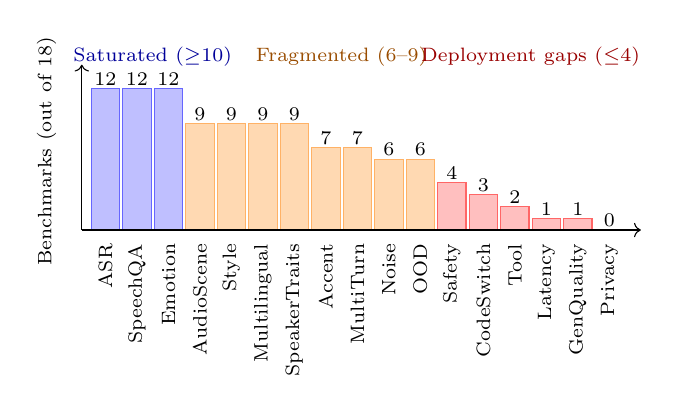
\begin{tikzpicture}[
  every node/.style={font=\footnotesize},
  bar/.style={fill=blue!25, draw=blue!60},
  bargap/.style={fill=orange!30, draw=orange!60},
  barlow/.style={fill=red!25, draw=red!60}
]
\foreach \i/\name/\count/\style in {
  1/ASR/12/bar,
  2/SpeechQA/12/bar,
  3/Emotion/12/bar,
  4/AudioScene/9/bargap,
  5/Style/9/bargap,
  6/Multilingual/9/bargap,
  7/SpeakerTraits/9/bargap,
  8/Accent/7/bargap,
  9/MultiTurn/7/bargap,
  10/Noise/6/bargap,
  11/OOD/6/bargap,
  12/Safety/4/barlow,
  13/CodeSwitch/3/barlow,
  14/Tool/2/barlow,
  15/Latency/1/barlow,
  16/GenQuality/1/barlow,
  17/Privacy/0/barlow
}{
  \ifnum\count>9
    \draw[bar] (\i*0.4-0.18,0) rectangle (\i*0.4+0.18, \count*0.15);
  \else\ifnum\count>4
    \draw[bargap] (\i*0.4-0.18,0) rectangle (\i*0.4+0.18, \count*0.15);
  \else
    \draw[barlow] (\i*0.4-0.18,0) rectangle (\i*0.4+0.18, \count*0.15);
  \fi\fi
  \node[rotate=90, anchor=east, font=\scriptsize] at (\i*0.4, -0.05) {\name};
  \node[font=\scriptsize] at (\i*0.4, \count*0.15+0.12) {\count};
}
\draw[->] (0.1,0) -- (7.2,0);
\draw[->] (0.1,0) -- (0.1,2.1);
\node[rotate=90, anchor=south, font=\scriptsize] at (-0.1,1.0) {Benchmarks (out of 18)};
\node[font=\scriptsize, blue!60!black]   at (1.0,2.2) {Saturated ($\geq$10)};
\node[font=\scriptsize, orange!60!black] at (3.4,2.2) {Fragmented (6--9)};
\node[font=\scriptsize, red!60!black]    at (5.8,2.2) {Deployment gaps ($\leq$4)};
\end{tikzpicture}
\caption{Capability coverage across 18 Speech LLM benchmarks
(2024--2026). Each bar shows how many benchmarks in our corpus
explicitly evaluate the capability. Coverage is dominated by ASR,
spoken question answering, and emotion; deployment-facing dimensions
(safety, code-switching, tool use, latency, generation quality,
privacy) remain weakly covered. The underlying 18~$\times$~17 coverage
matrix is released as supplementary material.}
\label{fig:benchmark_heatmap}
\end{figure}

The field is missing joint evaluation, not more benchmarks. A
capability may appear in several benchmarks while still being measured
under incompatible data sources, prompts, metrics, or judge protocols, and
the dimensions most needed for deployment (latency, safety, privacy,
generation quality) are precisely those least represented. We turn next to
whether even the dimensions that \emph{are} measured are measured
reliably.

\subsection{Methodological Validity: Data, Metrics, Judges, and Protocols}
\label{subsec:eval_validity}

The central issue is validity: whether a benchmark measures what it claims
to measure under conditions that support the conclusions being drawn. Four
forms of validity are especially relevant.

\paragraph{Construct validity.}
Construct validity asks whether the scoring method matches the target
capability. Multiple-choice formats, as in MMAU and AKB-2000
\cite{sakshi2024mmau,lu2026akb2000}, improve reproducibility but
underrepresent open-ended semantic behavior. Rule-based free-response
metrics such as WER, CER, F1, and ROUGE are objective but brittle under
paraphrase, script variation, and downstream task semantics. LLM-as-judge
scoring, used by AudioBench, VoiceBench, AIR-Bench, SD-Eval, and
SeaLLMs-Audio
\cite{wang2025audiobench,chen2024voicebench,yang2024airbench,ao2024sdeval,liu2025seallmsaudio},
better supports open-ended responses but introduces judge choice, prompt
sensitivity, and position-bias concerns formalized for text in
\cite{zheng2023judging}. SALMon \cite{maimon2024salmon} introduces a fifth
paradigm---modeling-based pairwise preference via likelihood
comparisons---that requires no external judge but is restricted to
relative comparisons. For subjective targets such as emotion and style,
single hard labels can be misleading because annotator disagreement is
part of the phenomenon. VoxEmo's distribution-aware metrics
\cite{zhang2026voxemo} therefore offer a principled direction for
paralinguistic evaluation, though the approach has so far been validated
on only two models (Qwen2-Audio and Audio Flamingo). The field needs
a second tier of metrics that match each capability's epistemic structure:
distributional for ambiguous targets, modeling-based for relative
comparison, and exact-match for pure information retrieval.

\paragraph{Ecological validity.}
Ecological validity asks whether benchmark data resembles real speech use.
Real recordings preserve speaker variability, disfluency, and spontaneous
acoustic artifacts, but they are costly and often have uneven demographic
coverage. Synthetic TTS data is scalable and controllable, enabling
benchmarks such as VoiceBench, StyleBench, VoiceAgentBench, and Audio2Tool
\cite{chen2024voicebench,zhao2026stylebench,jain2025voiceagentbench,pahwa2026audio2tool}
to cover many prompts or scenarios; however, synthetic speech may smooth
away idiosyncratic speaker behavior, fatigue, natural hesitation, and
real environmental variation. Hybrid designs that overlay perturbations
or scenes on real speech, as in SCENEBench and Hearing2Translate
\cite{iyer2026scenebench,papi2025hearing2translate}, are useful but still
require validation against natural recordings. We therefore propose
that synthetic-only benchmarks should not anchor deployment claims; any
fairness, robustness, or deployment claim should include a real-speech
validation slice.

\paragraph{Evaluator validity: judge agreement.}
Evaluator validity asks who or what judges the output. LLM judges make
large-scale open-ended evaluation feasible, but reported agreement with
humans is moderate rather than definitive. SD-Eval reports a Spearman
correlation $\rho = 0.613$ between GPT-4o judge scores and human ratings
\cite{ao2024sdeval}; SeaLLMs-Audio reports a Pearson correlation of 0.8
with 93\% agreement excluding ties \cite{liu2025seallmsaudio}; AIR-Bench
explicitly documents position bias and mitigates with answer-swap voting
\cite{yang2024airbench}; the canonical text-LLM judge-bias literature
\cite{zheng2023judging} confirms that these issues are systemic, not
benchmark-specific.

\paragraph{Evaluator validity: contamination risk.}
A more serious risk emerges when proprietary LLMs
help generate benchmark items, filter annotations, or score outputs. The
AKB-2000 paper \cite{lu2026akb2000} explicitly acknowledges that
proprietary LLMs co-curated its questions, capping their performance at
94--96\% as upper bound rather than independent measurement; FMSU-Bench
\cite{li2026fmsubench} uses Gemini 2.5 Pro as primary annotator with
multi-expert cross-validation; SeaLLMs-Audio uses Gemini-2.5-flash as
judge for the same model class. In each case a model's score may
partially reflect the curation pipeline rather than independent
capability. Human baselines remain limited: only three benchmarks in our
pool (MMAU, SD-Eval, SALMon) report human upper bounds at scale, making
it hard to interpret whether a given score indicates saturation,
progress, or metric artifact. We therefore propose that proprietary
judges should not score the same model family that helped curate the
benchmark, and that human baselines should accompany any new capability
claim.

\paragraph{Operational validity.}
Operational validity asks whether the benchmark reflects deployment. Many
benchmarks are valid for offline comparison but weak for choosing a
real-time voice assistant. Latency, streaming mode, endpointing, audio
chunking, hardware, batch size, interruption handling, and multi-turn
stability are rarely standardized alongside task accuracy. SCENEBench
\cite{iyer2026scenebench} is the only benchmark in the pool that
measures per-clip latency, and it does so in isolation from content
quality. VoiceAgentBench \cite{jain2025voiceagentbench} addresses tool
use but explicitly does not study dynamic real-time tool invocation.
This creates a deployment mismatch: benchmarks may report that a model
understands speech while remaining silent about whether it can respond
quickly, preserve paralinguistic cues, and remain safe during an
interactive session. We elaborate the latency and streaming dimensions
of this mismatch in Section~\ref{sec:deployment}. We therefore
propose that latency, streaming, and content quality should be jointly
reported, not separately.

\paragraph{Severity ranking.}
Among the four validity types, operational validity is the most damaging
for IPM-relevant deployment claims: a benchmark can score perfectly on
construct, ecological, and evaluator validity yet still fail to inform a
practitioner choosing a real-time voice system. Construct and evaluator
validity interact in direct tension---tightening one (e.g., requiring
distribution-aware scoring) often weakens the other (e.g., by demanding
LLM judges that cannot represent label distributions)---so they must be
balanced rather than maximized independently.

\subsection{Which Models Are Actually Evaluated? Reporting Bias and Deployment Mismatch}
\label{subsec:eval_models}

Existing benchmark surveys ask ``what does each benchmark cover?'' We
instead ask ``which models are systematically benchmarked, and which
remain invisible?'' The model-evaluation matrix concentrates around
accessible or widely recognized systems. Qwen2-Audio \cite{team2024qwen2}
appears in nine benchmarks; Whisper variants \cite{radford2023robust},
GPT-4o \cite{openai2024gpt4o}, and Whisper+LLM cascades each appear in
seven; Audio Flamingo \cite{kong2024audioflamingo} and Qwen2.5-Omni
\cite{xu2025qwen25omni} appear in six; SALMONN \cite{tang2023salmonn} and
LLaMA variants \cite{touvron2023llama} appear in five; pre-2.0 Qwen-Audio
\cite{bai2023qwen}, Gemini variants \cite{google2024gemini}, Qwen3-Omni
\cite{xu2025qwen25omni}, Mini-Omni \cite{xie2024miniomni}, Kimi-Audio
\cite{du2025kimiaudio}, and DeSTA2 \cite{lu2026desta2} each appear in
four. The concentration
is understandable: open-weight models are easier to run, Whisper cascades
serve as convenient baselines, and proprietary frontier models such as
GPT-4o and Gemini provide recognizable reference points.

This concentration creates reporting bias. Coverage of interaction-first
systems is sparse and asymmetric. Moshi \cite{défossez2024moshispeechtextfoundationmodel}
and the GPT-4o-Audio real-time mode each appear in a single benchmark
(VoiceBench \cite{chen2024voicebench}). Four other interaction-first
systems---MiniCPM-o 4.5, Voila, OmniFlatten, and Gemini Live
\cite{google2024gemini}---do not appear in any benchmark in our pool.
Ordinary GPT-4o or Gemini evaluations should be distinguished in
practice from evaluations of their real-time audio interaction
modes (the GPT-4o = 7 and Gemini = 4 counts in the matrix include
text-mode evaluations; real-time-audio-mode evaluation is essentially
absent from our pool). This is precisely the deployment regime that
motivates the Speech-LLM concept, and it is precisely the regime that
existing benchmarks fail to evaluate. We elaborate the deployment
implications of this gap in Section~\ref{sec:deployment}.

\subsection{Validity Gaps and Benchmark Design Principles}
\label{subsec:eval_gaps}

The four validity questions of Section~\ref{subsec:eval_validity} surface
four parallel gaps. The construct validity gap: benchmarks repeatedly
measure ASR, spoken QA, and emotion, but subjective and multi-channel
capabilities need metrics that preserve ambiguity and cross-channel
interaction. The ecological validity gap: synthetic data enables scale
but weakens real-world claims unless paired with real-speech validation.
The operational validity gap: latency, streaming, endpointing,
interruption handling, and multi-turn stability are not jointly
evaluated with content quality. The governance validity gap: safety,
privacy, speaker anonymity, provenance, and identity risks are
under-integrated into mainstream benchmark design and demand the
extended treatment in Section~\ref{sec:safety_privacy_governance}.

We propose five design principles for future Speech LLM benchmarks:

\begin{enumerate}
  \item \textbf{Multi-channel joint evaluation.} Each benchmark should
  report at least two of: content fidelity, paralinguistic awareness,
  interaction dynamics, latency, and safety. Audio2Tool's joint
  reporting of ASR, tool-use accuracy, and noise robustness
  \cite{pahwa2026audio2tool} is a partial precedent.
  \item \textbf{Distribution-aware scoring for subjective targets.}
  Emotion and style should use soft labels or distributional metrics
  when annotator disagreement is intrinsic, following VoxEmo's
  KLD/JSD/TVD template \cite{zhang2026voxemo}.
  \item \textbf{Cross-source validation.} Claims based mainly on
  synthetic speech should be replicated on real-speech subsets.
  SCENEBench's pairing of 16k synthetic and 20 natural validation
  clips \cite{iyer2026scenebench} illustrates the design pattern,
  though the natural-speech fraction remains negligibly small.
  \item \textbf{Mandatory evaluation metadata.} Reports should
  document prompts, judge model and version, decoding settings,
  hardware, audio chunking, streaming mode, and whether any LLM was
  used during data curation. Cross-domain work on model governance similarly suggests that validation artifacts should be assessed for stability rather than treated as one-off explanations, as shown by recent evidence on SHAP attribution instability in credit-risk modeling~\cite{lin2025shap}.
  \item \textbf{Speech-LLM Evaluation Cards.} Analogous to ML model
  cards \cite{mitchell2019modelcards}, each benchmark should publish
  a structured card declaring: (a) primary and secondary lenses from
  Table~\ref{tab:benchmark_taxonomy}; (b) capability cells from
  Figure~\ref{fig:benchmark_heatmap} that the benchmark measures;
  (c) data source (real, synthetic, hybrid); (d) scoring method
  (rule-based, LLM-judge with model and version, distribution-aware,
  modeling-based); (e) human baseline availability; (f) model
  coverage including any 0/$N$ omissions; and (g) acknowledged
  validity threats.
\end{enumerate}

\noindent Of these, Principle~1 is the most immediately actionable: it
requires no new dataset and can be retrofitted into current benchmark
releases by adding latency and safety metrics alongside existing
capability scores.

Evaluation is becoming a bottleneck for trustworthy Speech LLM
deployment. Current benchmarks reveal individual capabilities but
under-measure the interactions among speech content, timing,
paralinguistics, safety, and real-world use that voice systems must
handle simultaneously. The four validity gaps motivate the
deployment-oriented analysis in Section~\ref{sec:deployment} and the
safety-and-governance analysis in Section~\ref{sec:safety_privacy_governance}.
\FloatBarrier
\section{Deployment: From Capable Models to Real-Time Systems}
\label{sec:deployment}

The preceding section showed that the evaluation of Speech LLMs must account for multi-channel capabilities and interaction behavior. Deployment introduces a complementary question: whether these capabilities can be delivered continuously under low latency, bounded memory, and realistic hardware constraints. A model that performs well on offline ASR, TTS, or speech understanding benchmarks may still fail as an interactive system if it cannot process streaming input, emit partial output, handle long acoustic contexts, or operate within the resource limits of the target device.

The release of GPT-4o in mid-2024 made this deployment gap broadly visible~\cite{openai2024gpt4o}. It showed that low-latency spoken interaction with multimodal models could approach human conversational timing under the reported conditions: users could speak naturally, receive spoken responses with sub-second latency, and experience an interaction loop that was more fluid than those typically supported by earlier cascaded systems. GPT-4o therefore provides a useful user-experience reference point for the deployment literature: subsequent open, edge, and streaming systems study how parts of this experience can be supported under more transparent or resource-constrained settings. However, reproducing this experience remains difficult outside large proprietary systems. The bottleneck is not only model capability; it is also deployment.

Speech is harder to deploy than text because it is a continuous, multi-channel signal. A deployed Speech LLM must often listen while speaking, preserve linguistic content while tracking paralinguistic cues, produce partial outputs before an utterance is complete, and remain responsive under variable acoustic conditions. These requirements change the serving problem. Batch throughput is no longer sufficient; first-byte latency, token delay, memory growth, turn-taking stability, and edge feasibility become first-order metrics. This section reviews recent work that addresses these constraints through serving systems, deployment-oriented architectures, streaming inference, algorithmic acceleration, and full-duplex omni-modal design.

\subsection{The Deployment Predicament}

Classical speech pipelines separated ASR, dialogue modeling, and TTS. This separation made deployment modular: each component could be optimized and monitored independently. Speech LLMs collapse this boundary. A single model, or a tightly coupled model stack, may now perform recognition, reasoning, response planning, and speech generation. This integration can improve interaction quality, but it also makes deployment failures harder to isolate.

Five recurring deployment failure modes motivate the analysis in this section. The first is latency fragmentation: papers report time to first byte (TTFB), time to first token (TTFT), average token delay, end-to-end latency, or throughput, but these metrics capture different parts of the interaction loop. The second is streaming mismatch: models trained or evaluated on complete utterances are often adapted to streaming use only after training. The third is memory growth: long audio and video streams create key-value cache (KV-cache) and feature-cache pressure that differs from text-only contexts. The fourth is hardware mismatch: theoretical FLOPs do not reliably predict performance on CPUs, mobile NPUs, or mixed edge-cloud deployments. The fifth is interaction incompleteness: many systems optimize recognition or generation latency in isolation, but they do not evaluate simultaneous listening and speaking.

These failure modes show that deployment cannot be summarized by a single latency or throughput number. It depends on how model architecture, decoding policy, memory management, serving infrastructure, and hardware interact under realistic speech workloads.

\subsection{From Failure Modes to Deployment Analysis}

Assessing deployment work requires decomposing each claim into three parts: the operational pressure the system addresses, the system response it applies, and the runtime conditions that produce the result. This structure turns latency, streaming, memory, hardware, and interaction issues into concrete review questions. Does the system reduce first-response delay, incremental token delay, or complete-response time? Does it support partial input during generation? How does memory grow with audio duration? Which device, runtime stack, and serving policy produce the reported result?

The remainder of the section studies five system responses to these pressures: serving-system design, architecture-level deployment design, streaming inference, efficiency optimization, and full-duplex convergence. These responses are not mutually exclusive. A single Speech LLM service may combine a deployment-aware model, a streaming policy, cache and decoding optimizations, a serving stack, and a full-duplex interaction loop.

Table~\ref{tab:deployment-framework} turns this structure into a reporting checklist. The first two columns identify the deployment pressure behind each failure mode. The third column links that pressure to the design patterns most likely to affect it, and the final column specifies the conditions that a deployment card should record. The table is not a leaderboard and does not enumerate deployment papers; it defines the information required to interpret deployment claims in the systems discussed below.

\begin{table*}[t]
\centering
\footnotesize
\setlength{\tabcolsep}{3pt}
\begin{tabularx}{\textwidth}{>{\raggedright\arraybackslash}p{0.17\textwidth} >{\raggedright\arraybackslash}p{0.24\textwidth} >{\raggedright\arraybackslash}p{0.22\textwidth} X}
\toprule
Failure mode & System pressure & Relevant design pattern & Deployment criteria \\
\midrule
Latency fragmentation & First response, incremental output, and complete response measure different behaviors & Serving system; streaming inference & Report TTFB, token delay, end-to-end latency, streaming policy, and interaction-loop latency together. \\
Streaming mismatch & Complete-utterance models may behave differently under partial input & Streaming inference; architecture design & Separate offline and streaming settings; specify input chunk size, output granularity, and emission policy. \\
Memory growth & Long audio and video streams expand KV-cache, feature cache, and multimodal state & Efficiency optimization; serving system & Report input duration, output duration, cache policy, peak memory, and active compression or eviction methods. \\
Hardware mismatch & FLOPs and parameter count do not determine device-level behavior & Architecture design; serving system & Report device class, runtime stack, batch size, measured latency, measured memory, and edge/cloud placement. \\
Interaction incompleteness & Recognition or generation latency alone does not capture simultaneous listening and speaking & Full-duplex convergence; serving system & Evaluate simultaneous input/output, turn-taking, barge-in, interruption recovery latency, and response quality together. \\
\bottomrule
\end{tabularx}
\caption{A deployment analysis framework for Speech LLMs. Each failure mode induces a system pressure, points to relevant design patterns, and implies concrete criteria for deployment-card reporting.}
\label{tab:deployment-framework}
\end{table*}

The corresponding subsections discuss the quantitative signals reported by these systems. We do not aggregate them into a leaderboard because the systems differ in task, hardware, latency definition, and interaction setting.

\subsection{System-Level Serving}

System-level serving determines whether Speech LLM inference can run as temporal-stream execution rather than isolated prompt processing. The central design question is how to coordinate input ingestion, acoustic encoding, language generation, speech synthesis, customization, and cluster scheduling under one serving loop while controlling latency fragmentation, memory growth, hardware mismatch, and interaction incompleteness.

VoxServe (Kamahori et al., 2026) introduces a serving system designed specifically for Speech Language Models~\cite{kamahori2026voxserve}. Its main architectural idea is a model-execution abstraction that separates model architecture from system-level optimization. Modern SpeechLMs vary widely in their internal structures, including encoder-decoder ASR models, autoregressive speech generators, and codec-based synthesizers. Nevertheless, they share computational patterns such as attention over temporal sequences, streaming I/O, and multi-stage processing. VoxServe exploits these shared patterns to support streaming-aware scheduling and an asynchronous inference pipeline, reporting 10--20x higher throughput than existing implementations at similar latency across several modern SpeechLMs.

NIM4-ASR (Xie et al., 2026) studies serving from the perspective of model-system co-design~\cite{xie2026nim4asr}. Instead of asking how to serve an arbitrarily large model efficiently, it asks what model size is sufficient for production-grade quality and how such a model should be served at scale. The resulting system uses a 2.3B-parameter encoder-LLM architecture with a clear division of labor: the encoder handles acoustic processing, while the LLM handles linguistic reasoning. The production system supports real-time streaming inference and million-scale hotword customization through retrieval-augmented generation (RAG) with sub-millisecond retrieval latency.

EPD Disaggregation (Singh et al., 2025) extends the prefill-decode disaggregation paradigm from text LLMs to multimodal serving~\cite{singh2025epd}. Its main observation is that multimodal models introduce a separate bottleneck: encoding multimedia inputs such as video frames and audio spectrograms is expensive and operates on a different timescale from prefilling or token generation. The system separates serving into three independently scheduled phases, Encode, Prefill, and Decode, and adds a caching mechanism for multimedia tokens.

Evaluating Kubernetes Performance for GenAI Inference (Malleni et al., 2026) studies the infrastructure layer and reports substantial improvements in tail TTFT latency under Kubernetes-native routing and scheduling configurations, with the exact percentage depending on the metric and experimental setting~\cite{malleni2026kubernetes}. Although this work is not specific to Speech LLMs, it is relevant because speech interaction is highly sensitive to tail latency.

The shared pattern is that serving decisions determine which part of the speech interaction loop becomes visible. VoxServe emphasizes heterogeneous temporal execution, NIM4-ASR emphasizes the production ASR boundary between acoustic encoding and linguistic reasoning, EPD Disaggregation emphasizes phase separation, and Kubernetes-level work emphasizes cluster behavior. Speech LLM deployment needs serving stacks that expose throughput, TTFT, and interaction-level traces under the same setup, including simultaneous input ingestion, output generation, interruption handling, cache growth, and tail latency under realistic audio durations.

\subsection{Architecture-Level Deployment Design}

Architecture-level work brings deployment constraints into the model design stage. Instead of treating latency, memory, and hardware behavior only as serving issues, these systems make them part of the architecture itself. This premise is especially important for edge and consumer hardware, where memory and latency limits cannot be addressed only through better serving.

LFM2 (Amini et al., 2025) uses hardware-in-the-loop architecture search under explicit edge latency and memory constraints~\cite{amini2025lfm2}. The resulting hybrid backbone combines gated short convolutions with grouped query attention blocks and is optimized for measured performance on target hardware rather than theoretical FLOPs. The model family ranges from 350M to 8.3B parameters, includes dense and MoE variants, supports 32K context length, and is trained on 10--12 trillion tokens. The LFM2-Audio variant supports real-time speech-to-speech interaction, reports competitive quality relative to substantially larger models under its evaluation setting, and achieves 2x faster prefill and decode on CPUs than similarly sized models.

MiniCPM-o 4.5 (Cui et al., 2026) focuses on full-duplex interaction~\cite{cui2026minicpmo}. Many multimodal models still operate in alternating phases: they perceive and then respond. This design prevents the model from incorporating new inputs during generation or acting proactively. MiniCPM-o introduces Omni-Flow, a streaming framework that aligns omni-modal inputs and outputs on a shared temporal axis and transforms turn-based interaction into continuous, time-aligned processing. With 9B parameters and less than 12GB RAM, it is presented as an open-source model that supports simultaneous seeing, listening, and speaking with proactive behavior on consumer edge hardware.

S2M3 (Yoon et al., 2025) takes a modular approach to edge deployment by decomposing multi-modal models into reusable modules for distributed multi-task inference~\cite{yoon2025s2m3}. By allowing the same encoder modules to serve multiple downstream tasks, S2M3 reduces memory use by up to 62\% and improves latency by 56.9\% relative to cloud-based approaches. TinyM2Net-V3 (Rashid \& Mohsenin, 2024) studies a more constrained setting, combining knowledge distillation with low-bit-width quantization for multimodal audio-visual inference under severe memory limits~\cite{rashid2024tinym2net}.

These systems represent four distinct deployment philosophies. LFM2 optimizes directly for measured hardware behavior, MiniCPM-o optimizes for interaction continuity, S2M3 optimizes for modular resource sharing, and TinyM2Net-V3 targets severe memory constraints through compression. Together, they show that deployment-aware architecture design spans trade-offs among latency, memory, modularity, and interaction capability. Speech LLM deployment needs architecture specifications that include device class, measured latency, memory footprint, supported context length, input audio duration, and output audio duration.

\subsection{Streaming and Real-Time Inference}

Streaming work makes output timing part of the inference objective. A streaming model must decide not only what to output, but also when to output it. Component-level latency and conversational-loop latency are related but not identical: a correct response that arrives too late may still fail the interaction.

Ultra-Low Latency End-to-End Streaming Speech Synthesis (Su et al., 2026) reports 48.99ms average TTFB and 10.6x acceleration over conventional cascaded pipelines under its evaluation setting~\cite{su2026ultralowtts}. The key idea is to remove the vocoder bottleneck by directly modeling the compressed discrete latent space of the Mimi neural audio codec. A modified FastSpeech 2 backbone uses progressive depth-wise sequential decoding across 32 residual vector quantization layers to generate speech in non-autoregressive blocks. Experiments in English and Malay provide cross-language evidence within the scope of the evaluated languages.

SpeakStream (Bai et al., 2025) addresses the LLM-then-TTS cascade used in many conversational AI systems~\cite{bai2025speakstream}. Traditional TTS models are trained on complete utterances and can introduce large delays when paired with streaming LLM text. SpeakStream uses a decoder-only architecture trained with next-step prediction on interleaved text-speech data, enabling it to generate audio incrementally while receiving streaming text.

Streaming ASR with Decoder-Only LLMs (Wan et al., 2026) studies when an LLM-based ASR system should emit tokens relative to the input speech~\cite{wan2026streamingasr}. A read/write policy network with monotonic chunkwise attention reduces average token generation delay by 62.5\% under the reported setup. Mini-Omni (Xie \& Wu, 2024) was an early end-to-end system for real-time speech interaction without an external TTS system~\cite{xie2024miniomni}. Its text-instructed speech generation method, batch-parallel inference strategy, and ``Any Model Can Talk'' training method showed that a single model could handle the complete speech interaction loop while preserving core language capabilities.

The shared pattern is that different systems optimize different latency boundaries. TTFB, first-token latency, token generation delay, and end-to-end latency answer different questions. A speech synthesis result with strong TTFB and an ASR result with low token delay provide complementary views of latency, but neither metric alone characterizes the full interaction loop. Speech LLM deployment needs latency optimization at the conversational-loop level, where component latency links to streaming policy, input chunk size, output granularity, and downstream user-visible response time.

\subsection{Efficiency Optimization}

Efficiency optimization treats decoding, compression, and cache management as deployment levers that can control memory growth and hardware mismatch without redesigning the entire model or serving stack. Real systems may combine quantization, speculative decoding, cache pruning, batching, and streaming policies, so the important deployment question is how these gains interact when they are composed.

\subsubsection{Compression and Quantization}

Quantizing Whisper-small (Sohler et al., 2026) evaluates post-training quantization across libraries and bit-widths for Whisper and provides practical guidance for constrained hardware~\cite{sohler2025quantizingwhisper}. Edge-ASR (Feng et al., 2025) expands this analysis to eight post-training quantization (PTQ) methods across Whisper and Moonshine, and identifies best practices for low-bit edge deployment~\cite{feng2025edgeasr}. Resource-Efficient Speech Quality Prediction (Nilsson et al., 2024) shows that binary activation maps with 8-bit quantization-aware training (QAT) can reduce inference memory by 25-fold for speech quality assessment~\cite{nilsson2024speechquality}. These results suggest that speech models may tolerate aggressive quantization in some settings, but this tolerance depends on the task, architecture, and evaluation metric.

\subsubsection{Speculative Decoding}

Speculative decoding uses a fast draft model to propose tokens that a larger verifier accepts or rejects in parallel. SpecASR (Wei et al., 2025) reports 3.04--3.79x speedup over autoregressive decoding with no accuracy loss under its evaluation setting, using adaptive draft generation and a sparse token tree~\cite{wei2025specasr}. Accelerating Autoregressive Speech Synthesis (Lin et al., 2025) applies speculative decoding to TTS and reports a 1.4x speedup while maintaining fidelity and naturalness~\cite{lin2025speechspeculative}. The smaller gain relative to ASR is consistent with the higher token entropy of speech synthesis.

Edge-Cloud Collaborative Speech Emotion Captioning (Xue et al., 2026) introduces Uncertainty-Guided Speculative Decoding for privacy-preserving edge-cloud collaboration~\cite{xue2026edgecloudsec}. A lightweight edge model drafts emotion captions locally, and only high-uncertainty token blocks are sent to a cloud verifier. Model-free Speculative Decoding (Ho et al., 2025) removes the draft model and instead uses precomputed n-gram token maps, reporting a 10\% absolute speed improvement on CPU with minimal additional memory~\cite{ho2025modelfreeasr}.

\subsubsection{KV-Cache Optimization}

AccKV (Jiang et al., 2025) addresses KV-cache growth in audio-video LLMs, where both modalities create long temporal sequences~\cite{jiang2025acckv}. The key observation is that attention in higher transformer layers shifts toward the video modality regardless of task type. AccKV uses Layer Adaptive Focusing to identify important tokens by layer and modality, and Cross-Calibration to align low-priority modality caches with high-priority ones before selective eviction.

Across these studies, the shared pattern is modular efficiency: each method improves one pressure point in the deployment stack. Speech LLM deployment needs to treat these methods as composable system policies rather than isolated speedups. For example, evaluations can combine quantization, speculative decoding, and cache pruning under the same streaming input regime. This is the deployment analogue of evaluating individual benchmark capabilities together rather than only in isolation.

\subsection{Deployment Evidence Under Realistic Pressure}

Deployment evidence should specify whether a result comes from a product demonstration, a reproducible component benchmark, or a controlled system measurement. GPT-4o-like products define compelling user-facing targets, while open systems make instrumentation, ablations, and controlled measurement easier. Researchers often study Whisper-derived ASR models, codec-based TTS pipelines, and selected open multimodal models because these systems support reproducible instrumentation. Interaction-first systems such as MiniCPM-o 4.5, OpenOmni, GPT-4o-Audio-style real-time systems, and Gemini Live-style products provide references for interaction quality, although access, instrumentation, and reproducibility differ across systems.

Speech LLM deployment needs to separate three kinds of evidence: product-level demonstrations, reproducible component benchmarks, and controlled system measurements. Product demonstrations define experience targets; component benchmarks isolate mechanisms; controlled system measurements compare deployment behavior. Treating these as complementary forms of evidence makes cross-system comparison clearer without using one form as a substitute for another.

\subsection{Full-Duplex and Omni-Modal Convergence}

Full-duplex omni-modal systems treat perception and generation as concurrent rather than alternating processes. Full-duplex interaction is therefore not merely faster streaming; it changes the interaction contract. A system must process incoming audio or visual streams while generating speech, maintain low latency in both directions, accept interruptions, and coordinate multiple modalities under memory and compute constraints.

OpenOmni (Luo et al., 2025) introduces a two-stage progressive multimodal alignment framework with 7B parameters~\cite{luo2025openomni}. A notable result is cross-modal transfer: training a pre-trained speech model on text-image tasks yields near-zero-shot generalization from vision to speech and outperforms models trained on explicit tri-modal datasets. A lightweight non-autoregressive decoder trained with direct preference optimization produces real-time emotional speech with sub-1-second latency and a 5x speedup over autoregressive methods. Together with MiniCPM-o 4.5, OpenOmni illustrates a broader trend toward omni-modal models in the 7--9B range that can run on consumer hardware with real-time responsiveness.

This convergence changes the deployment target. The field no longer only needs faster ASR, faster TTS, or cheaper serving; it needs an interaction loop in which perception, reasoning, and speech generation occur continuously. Speech LLM deployment should treat full-duplex interaction as a first-class target and measure turn-taking, barge-in, interruption recovery latency, memory growth, and content quality together because these properties determine whether a system remains responsive and coherent during overlapping input and output.

\subsection{Deployment Recommendations}

Speech LLM deployment should design, optimize, and describe systems as real-time interaction loops rather than as independent ASR, LLM, and TTS components. Speculative decoding, quantization, KV-cache pruning, streaming serving, and edge deployment all improve different pressure points, but their value is clearest when they are tied to the deployed interaction regime.

First, deployment should move from isolated optimization to composed optimization. When a system combines quantization, speculative decoding, cache pruning, batching, or streaming policies, the evaluation should treat these choices as one deployment configuration whose combined behavior determines latency, quality, and memory growth.

Second, deployment should make streaming state explicit. Input chunk size, output granularity, cache policy, audio duration, interruption setting, and simultaneous input-output status define the runtime state of a Speech LLM. These details connect component speedups to the actual interaction loop.

Third, deployment should align latency metrics with interaction conditions. TTFB, average token delay, end-to-end latency, and time-to-completion each characterize a different user-visible behavior: first response, incremental output, complete answer delivery, or interruption recovery.

A deployment card summarizes these recommendations as a compact disclosure of the operational conditions under which an evaluation measures a deployment claim. At minimum, it should include model size, hardware, batch size, streaming policy, input duration, output duration, active optimizations, latency metric, quality metric, baseline implementation, and whether the evaluation uses cloud, edge, streaming, or full-duplex settings. This practice makes cross-paper comparison more tractable even when tasks differ.

The broader recommendation is to report both component-level measurements and interaction-loop measurements. A low TTFB becomes more interpretable when the evaluation connects it to conversational responsiveness. Similarly, evaluations should tie ASR token delay to downstream response delay when the target application is an assistant or agent. For full-duplex systems, evaluation should measure turn-taking, interruption handling, latency, and content quality together. This is the deployment counterpart of multi-channel evaluation: the system must be correct, responsive, and stable at the same time.

These deployment choices also determine the safety surface of Speech LLMs. Systems that stream continuously, retain acoustic context, split computation across edge and cloud, or synthesize speech in real time expose new risks related to privacy, impersonation, provenance, and audio-specific attacks. Section~\ref{sec:safety_privacy_governance} turns to these safety, privacy, and governance implications.

\section{Safety, Privacy, and Governance}
\label{sec:safety_privacy_governance}

Speech Large Language Models (Speech LLMs) extend language-model interaction from text to spoken communication, but this shift also changes the safety and privacy problem. Speech is not simply text represented as audio. It can serve as a command channel, an acoustic signal, a marker of speaker identity, and a carrier of synthetic media. A spoken utterance may encode words, speaker characteristics, prosody, emotion, accent, background sounds, and signal-level artifacts. These properties make speech useful for natural interaction, but they also create attack and misuse pathways that are not captured by text-only safety evaluation.

This section reviews six groups of risks and mitigations: input-side audio jailbreaks and adversarial speech, audio safety benchmarks, guardrails and anti-cloning defenses, synthetic voice misuse, speaker privacy protection, and documentation for governance. Because many of the cited studies are recent preprints, their findings should be interpreted cautiously. Still, the literature points to a consistent pattern: safeguards developed for text-only LLMs do not necessarily transfer to speech-capable systems. Speech LLMs therefore require safety analysis that accounts for audio representations, speech generation, speaker identity, and deployment context.

\subsection{Speech-Specific Risk Surface}

Speech LLMs expose semantic, acoustic, biometric, and synthetic-media risks at the same time. In text-only LLMs, harmful prompts are usually represented as discrete text tokens. In Speech LLMs, the input may pass through raw waveform encoders, speech tokenizers, ASR modules, acoustic projectors, or multimodal alignment layers before reaching the language backbone. These processing stages can change model behavior and create attack opportunities that are difficult to detect from transcripts alone. Recent AI-ethics work argues that audio language model deployments should be scoped by a principle of least privilege---granting a system access only to the acoustic information a task actually requires---precisely because raw audio carries far more than the intended semantic payload \citep{he2025modelhears}.

\subsubsection{Input-Side Attacks: Harmful Spoken Prompts and Modality Transfer Failure}

Red-teaming studies show that safety behavior can change when harmful requests are presented as speech rather than text. \textbf{Audio Is the Achilles' Heel} evaluates Qwen-Audio, Qwen2-Audio, SALMONN-7B, SALMONN-13B, and Gemini-1.5-Pro under three settings: harmful questions in text and audio formats, harmful text paired with distracting non-speech audio, and speech-specific jailbreaks. Beyond aggregate attack success, the paper analyzes representation-space behavior using t-SNE visualizations and response-opening patterns. The authors find that harmful questions can become more effective when moved into the audio modality for several open-source audio LMMs, and that non-speech audio can reshape representation spaces in ways that affect safety behavior \citep{yang2024audioachillesheelred}. This result suggests that safety alignment learned through text may weaken after multimodal adaptation.

Adversarial audio attacks further show that the waveform itself can be optimized to bypass safety constraints. \textbf{AdvWave} treats jailbreak attacks against large audio-language models as a waveform-level optimization problem. The method includes dual-phase optimization to address gradient shattering from audio encoder discretization, adaptive target search to handle response variability, and classifier-guided natural-sound constraints to keep perturbations perceptually plausible \citep{kang2024advwavestealthyadversarialjailbreak}. This matters because the attack can operate below the transcript level: the spoken request may remain understandable to humans, while the acoustic perturbation changes how the model processes or answers it.

Multimodal attacks add another path. \textbf{JAMA} proposes a joint audio-text attack against spoken language models by combining gradient-based text suffix optimization with audio perturbation. The method jointly optimizes across modalities and evaluates both fixed-prompt and prompt-adjusted settings. Experiments show that combined text-audio attacks can outperform unimodal attacks across several spoken language models \citep{krishnan2026optimizingmultimodaljailbreaksspoken}.

Sparse token attacks show that only parts of the audio sequence may be sufficient for a successful jailbreak. \textbf{TAGO} analyzes token-aligned gradients and finds that gradient energy is not evenly distributed across audio tokens. Its method identifies high-contribution token regions and optimizes only the corresponding waveform segments. Comparisons with full-waveform attacks, token-selection strategies, and efficiency analyses show that sparse token optimization can reduce attack cost while maintaining strong jailbreak performance \citep{fang2026sparsetokenssufficejailbreaking}. This suggests that small local changes in audio should not be treated as automatically harmless.

Across these attacks, harmfulness is no longer only a property of the transcript. It can be introduced, strengthened, or hidden through the acoustic path. A speech-specific threat model should therefore include harmful spoken prompts, distracting non-speech audio, adversarial waveform perturbations, multimodal audio-text jailbreaks, speech-specific jailbreak prompts, and sparse token-level manipulation.

\subsubsection{Output-Side Misuse: Synthetic Voice and Impersonation}

Speech generation introduces a different class of risk. A generated voice can carry both content and an apparent speaker identity. Voice cloning is therefore more than harmful text generation with audio output; it can support impersonation, fraud, reputational harm, evidence manipulation, and social engineering. A speech assistant that can listen, reason, act, and reply in a realistic voice may improve accessibility and interaction, but it can also scale impersonation if voice generation is not constrained.

Voice cloning misuse can be grouped into three categories:

\begin{itemize}
\item \textbf{Identity impersonation:} a malicious actor uses a cloned voice to appear to be another person.
\item \textbf{Evidentiary manipulation:} synthetic audio is presented as proof that someone said something.
\item \textbf{Social engineering:} a cloned voice increases trust in scams, phishing, coercion, or fraudulent instructions.
\end{itemize}

Each category calls for different controls. Identity impersonation requires consent and anti-cloning protection; evidentiary manipulation requires provenance and forensic verification; social engineering requires organizational procedures such as callback verification, transaction limits, and human review.

\subsubsection{Privacy Leakage: Speaker Identity and Paralinguistic Attributes}

Speech privacy extends beyond the literal words being spoken. Even benign speech can reveal speaker identity, accent, age, emotional state, or background context. Speech LLMs that process raw or lightly processed audio may therefore collect more personal information than the user intended to provide. Stored audio and speaker embeddings can also become biometric records that later enable identity recovery or voice cloning.

This distinction separates two related risks. Voice cloning and deepfakes concern synthetic speech as an output misuse problem. Speaker privacy concerns risks that arise from the user's input speech, even when the content is harmless. Raw audio, voice embeddings, transcripts, and paralinguistic features can all contribute to identity leakage. Speech LLM systems should therefore treat speech as both conversational content and personal data.

\subsection{Audio Safety Evaluation and Benchmarking}

As audio jailbreak methods become more varied, benchmark design becomes central to safety evaluation. Early demonstrations often used small prompt sets or single-model case studies. Newer benchmarks aim to test attacks, models, defenses, perturbations, and evaluation protocols under more controlled settings.

\subsubsection{Unified Jailbreak Benchmarks}

\textbf{JALMBench} provides a broad framework for evaluating jailbreak vulnerabilities in large audio-language models. Its dataset includes harmful query samples, text-transferred jailbreak samples, and audio-originated jailbreak samples. It synthesizes audio variants with different accents, genders, TTS methods, and languages, and evaluates multiple LALMs across several attack and defense methods. The paper also reports evaluator reliability analysis, including repeated judging, cross-model consistency, and human consistency verification \citep{peng2026jalmbenchbenchmarkingjailbreakvulnerabilities}. These details are important because benchmark results depend not only on the prompt set, but also on how harmfulness is judged.

The JALMBench results support several design lessons. Non-adversarial harmful queries can have different attack success rates in text and audio modalities. Stronger attacks such as AdvWave can achieve high attack success under the benchmark's settings. Topic sensitivity, attack efficiency, voice diversity, and architecture effects can all influence safety outcomes. These findings suggest that safety evaluation should report accent, speaker, and language variation explicitly, because robustness observed under one speech variety may not generalize to another \citep{peng2026jalmbenchbenchmarkingjailbreakvulnerabilities}.

\subsubsection{Perturbation-Based Benchmarking}

\textbf{Audio Jailbreak} provides a complementary benchmark focused on realistic speech and perturbation. Its base dataset converts adversarial text prompts into speech across policy-violating categories. The paper also introduces an Audio Perturbation Toolkit that applies transformations in the time, frequency, and amplitude domains while aiming to preserve semantic consistency. These transformations test whether safety behavior remains stable under speed changes, noise, clipping, pitch shifts, and related distortions \citep{song2025audiojailbreakopencomprehensive}. This matters because deployed speech systems rarely receive clean, studio-quality audio.

\textbf{Jailbreak-AudioBench} combines a toolbox, dataset, and benchmark for studying audio jailbreaks. It introduces explicit and implicit jailbreak audio examples and evaluates multiple large audio-language models. One contribution is its focus on audio editing as a jailbreak mechanism: harmful semantics can be embedded or transformed through audio operations rather than simply read aloud as a standard prompt \citep{cheng2026jailbreakaudiobenchindepthevaluationanalysis}. This is especially relevant for end-to-end Speech LLMs, which may preserve acoustic information that cascaded ASR-to-LLM systems discard.

\subsubsection{Evaluation Requirements}

Across these benchmark papers, several evaluation requirements emerge:

\begin{itemize}
\item Models should be tested on clean harmful spoken prompts.
\item Models should be tested on perturbed harmful prompts.
\item Benchmarks should include text-transferred and audio-originated jailbreaks.
\item Evaluation should include multimodal audio-text attacks.
\item Speaker, accent, language, and environmental variation should be reported.
\item Defenses should be evaluated together with benign utility.
\end{itemize}

The benchmark gap is therefore not only about dataset size. Audio safety scores depend on perturbation choices, voice diversity, judge stability, target-model assumptions, and benign-utility trade-offs. Benchmark papers should report target models, judges, safety categories, attack assumptions, and whether evaluation relies on human review, model-based judging, or rule-based filtering.

\subsection{Mitigation: Guardrails, Anti-Cloning, and Privacy Defenses}

The attack and benchmark literature shows that text-only moderation is insufficient for Speech LLMs. If an attack is encoded in the acoustic signal, a filter applied only to the transcribed text may miss it. If a system removes too much acoustic information before model processing, it may also harm useful capabilities such as accent robustness, emotion understanding, speaker adaptation, or paralinguistic reasoning. Mitigation therefore has to cover jailbreak guardrails, anti-cloning defenses, privacy protection, and deployment monitoring.

\subsubsection{Audio-Language Guardrails}

\textbf{ALMGuard} provides one example of an audio-language-specific defense. The paper argues that defenses transferred from traditional audio adversarial attacks or text jailbreak defenses are limited against ALM-specific threats. The method identifies safety shortcuts in model activations and introduces safety shortcut activation perturbations as a runtime defense. It also uses a Mel-Gradient Sparse Mask to preserve benign utility. The paper evaluates the defense against multiple attack methods and includes analyses of benign task preservation \citep{jin2025almguardsafetyshortcutsguardrails}. This supports the need for guardrails that operate at the representation or activation level, not only at the transcript level.

Current guardrail research does not yet cover all parts of the threat model equally. Speech-specific jailbreak prompt transformations and sparse token-level manipulation remain only partially addressed by existing defenses. Future defenses may need to combine input detection, token-level robustness analysis, activation-level guardrails, and output monitoring.

\subsubsection{Anti-Cloning Defenses}

For speech synthesis and voice cloning, defenses must also address output-side misuse. \textbf{E2E-VGuard} focuses on unauthorized voice cloning in production LLM-based end-to-end speech synthesis. The paper's threat model describes API-based cloning workflows in which users upload only audio, while the platform internally performs ASR and TTS training. The method protects both timbre and pronunciation: timbre protection uses an encoder ensemble and MFCC-based feature loss to reduce speaker similarity in synthesized audio, while pronunciation protection attacks ASR transcription so that fine-tuning receives incorrect text-audio pairs. The paper also uses a psychoacoustic model to keep perturbations difficult for humans to perceive and evaluates across open-source synthesizers, commercial APIs, ASR systems, languages, and speakers \citep{zhang2025e2evguardadversarialpreventionproduction}. This shows that anti-cloning defense has to consider the full speech synthesis pipeline, not only the final waveform.

\subsubsection{User-Side Voice Privacy Protection}

User-side privacy protection is another defense direction. \textbf{Enkidu} proposes real-time audio privacy protection against personalized voice deepfake threats using universal frequency-domain perturbations. The method does not assume white-box access to the attacker's cloning model. Instead, it uses black-box knowledge, few-shot training, and frequency-domain perturbations designed to preserve perceptual quality while reducing cloneability. The experiments evaluate privacy protection, audio quality, real-time efficiency, and robustness across settings \citep{feng2025enkiduuniversalfrequentialperturbation}. This is relevant for users who want to publish or transmit speech while reducing the risk that their voice can later be cloned.

\subsubsection{Adaptive De-Anonymization and Purification Attacks}

Privacy defenses should be evaluated against adaptive attackers. \textbf{VoxATtack} studies a multimodal attack against voice anonymization systems. Its key insight is that anonymized speech may still leak identity when acoustic and textual information are combined. The method extracts both acoustic embeddings and text embeddings, then fuses them for de-anonymization. Experiments against VoicePrivacy benchmark settings show that multimodal attacks can outperform acoustic-only baselines \citep{aloradi2026voxattackmultimodalattackvoice}. For Speech LLMs, this is important because these systems often process both audio and text representations. Even if the voice is transformed, the transcript may contain linguistic habits, topic choices, names, or discourse patterns that help re-identify the speaker.

\textbf{VocalBridge} further challenges perturbation-based privacy defenses. The paper studies an adaptive attacker who purifies protected speech before using it for voice cloning or speaker verification. Its method uses a diffusion-bridge model in the EnCodec latent space to map protected speech back toward clean speech, with an optional Whisper-guided phoneme conditioning variant. The paper defines user objectives such as imperceptibility, verifiability, and inimitability, and attacker objectives such as restoring verifiability and breaking inimitability. Its evaluation across proactive defenses, voice synthesis tools, and speaker verification systems suggests that perturbation-based protections may be fragile against purification \citep{abbasihafshejani2026vocalbridgelatentdiffusionbridgepurification}.

\subsubsection{Layered Defense Architecture}

A practical mitigation architecture for Speech LLMs should include several layers:

\begin{itemize}
\item \textbf{Input-level defenses:} inspect audio for suspicious transformations, hidden instructions, adversarial perturbations, or abnormal acoustic patterns.
\item \textbf{Representation-level defenses:} monitor acoustic embeddings or hidden states for attack-like behavior.
\item \textbf{Transcription-level defenses:} inspect ASR output while recognizing that transcription is not sufficient on its own.
\item \textbf{Output-level defenses:} moderate generated text and generated speech before delivery.
\item \textbf{Privacy controls:} minimize raw audio storage, separate content processing from identity processing, and document whether speaker embeddings are stored.
\item \textbf{Deployment-level controls:} include logging, rate limits, human escalation, and incident response for high-risk applications.
\end{itemize}

These defenses shift Speech LLM safety from a single-filter problem to a layered systems problem. Because attacks may target the waveform, transcript, internal representation, generated speech, or deployment workflow, defenses should be tested under adaptive conditions.

\subsection{Identity Misuse and Synthetic Speech Provenance}

Synthetic speech risks are related to privacy risks, but they are not the same. The previous subsection focused on defenses against jailbreaks, cloning, and identity leakage. This subsection focuses on generated speech after it leaves the model: whether it can be detected, attributed, and traced.

\subsubsection{Deepfake Detection Under Realistic Conditions}

The \textbf{Perturbed Public Voices (P$^{2}$V)} dataset examines the weakness of audio deepfake detectors under realistic conditions. Its dataset includes identity-consistent transcripts, environmental and adversarial noise, and voice cloning systems from multiple years. The paper evaluates several detectors and shows that performance drops under stronger perturbations and newer cloning methods \citep{gao2025perturbedpublicvoicesp2v}. This supports the argument that deepfake detection should not be validated only on clean or closed-set benchmarks. Speech LLM governance should assume that generated or cloned audio may be compressed, re-recorded, mixed with background noise, or produced by newer synthesis systems than those seen during detector training.

\subsubsection{Robustness Limits of Audio Watermarking}

Watermarking and provenance mechanisms help identify AI-generated speech and support misuse investigation. However, audio can be compressed, resampled, re-recorded, denoised, edited, cropped, transformed by neural codecs, or regenerated by another model. Each operation can weaken or remove a watermark.

A systematic study of audio watermark robustness surveys 22 watermarking schemes and evaluates removal attacks across signal-level, physical-level, and AI-induced distortions. The paper categorizes watermarking approaches, builds an evaluation pipeline, and tests robustness under many removal configurations. The authors conclude that no surveyed scheme is robust against all tested distortions in practice \citep{wen2025sokrobustaudiowatermarking}. This is a caution for Speech LLM deployment: watermarking can support provenance, but it cannot be the only safeguard.

\textbf{Deep Audio Watermarks are Shallow} focuses on limitations of post-hoc speech watermarking. The paper analyzes how post-hoc methods manipulate low-level audio features after generation and shows that transformation-based removal can reduce detectability while preserving audio quality. Its evaluation shows why watermark robustness depends on the attacker's ability to process or transform the signal without knowing the watermarking scheme \citep{oreilly2025deepaudiowatermarksshallow}. This suggests that post-hoc watermarking should be supplemented by generation-time provenance, secure metadata, or model-integrated methods.

\subsubsection{Generation-Time and Dual-Provenance Watermarking}

Several newer methods propose stronger watermarking strategies. \textbf{MelShield} embeds keyed payloads into Mel-spectrogram representations during TTS generation. Its method integrates watermarking into the TTS pipeline rather than relying only on post-processing, and its experiments evaluate attribution accuracy, robustness, and audio quality. This is useful for Speech LLMs because speech generation systems often operate through intermediate acoustic representations such as Mel-spectrograms, making internal watermarking more natural than waveform-only post-processing \citep{jin2026melshieldrobustmeldomainaudio}.

\textbf{DualMark} extends provenance from model-level attribution to both model and training-data attribution. The paper defines a dual-level attribution problem, embeds model and data watermarks into Mel-spectrogram representations during training, and uses watermark consistency loss so generated audio preserves decodable provenance. Its experiments compare model-level and data-level attribution, ablate the watermark consistency loss, and evaluate robustness against pruning, compression, resampling, and noise \citep{yang2025dualmarkidentifyingmodeltraining}. This is relevant because accountability may require identifying both the generating model and the data source.

\textbf{AWARE} proposes watermarking through adversarial resistance to edits. Its method is designed around the possibility that watermarked audio may be edited, cropped, compressed, or desynchronized. Instead of relying only on fixed simulated distortions, it trains the watermarking system with adversarial resistance and uses a detector that aggregates temporal evidence. This direction is important because synthetic speech may be transformed many times before detection \citep{pavlović2026awareaudiowatermarkingadversarial}.

The watermarking literature reframes provenance as a robustness-under-transformation problem. The question is not only whether a watermark can be detected on clean generated audio, but whether it survives compression, re-recording, editing, adversarial removal, and model-based transformation.

\subsubsection{Traceability Stack}

For Speech LLM deployment, provenance should be treated as a stack rather than a single watermark. A traceability system may include:

\begin{itemize}
\item Audio watermarking.
\item Secure metadata.
\item Model version records.
\item Consent records.
\item User identity verification for voice cloning.
\item Audit logs and incident response procedures.
\end{itemize}

In public-facing or high-risk settings, generated speech should remain traceable even when the audio watermark fails. The secure-metadata layer is now being standardized outside the research literature: the C2PA Content Credentials specification attaches cryptographically signed provenance manifests to media, and news organizations have begun deploying it against deepfakes and disinformation \citep{strickland2024credentials}. Watermarking is useful but insufficient: it supports accountability, but it has to be combined with such signed metadata, policy, monitoring, and operational safeguards.

\subsection{Governance, Documentation, and Compliance Gaps}

The traceability stack above describes technical provenance mechanisms. This subsection turns to documentation and governance. Speech LLMs need documentation that covers not only model accuracy, but also intended use, prohibited use, data provenance, speaker privacy, audio safety testing, watermarking, logging, and incident response. General AI governance frameworks provide useful starting points, but they need speech-specific extensions. Recent policy scholarship on generative-AI governance emphasizes that effective regimes must span the full model lifecycle---development, deployment, and post-deployment monitoring---rather than regulating a single release point \citep{taeihagh2025governance}, a lifecycle view that maps directly onto the speech-specific requirements below.

\subsubsection{Model Documentation}

\textbf{Model Cards} offer a starting point for standardized model reporting. The paper proposes short documents accompanying trained models, including intended use, performance evaluation, ethical considerations, and performance across relevant groups and conditions. Although the original framework focuses on machine learning models more broadly, the same structure can be adapted to Speech LLMs \citep{mitchell2019modelcards}. A Speech LLM model card should report supported languages and accents, evaluated noise conditions, speech input and output capabilities, audio jailbreak testing, deepfake risk controls, privacy protections, latency constraints, and whether raw audio or speaker embeddings are stored.

\subsubsection{Machine-Readable Governance}

Machine-readable documentation may help connect policy requirements to system behavior. \textbf{AI Cards} propose human- and machine-readable documentation for AI systems, including technical specifications, context of use, and risk management information inspired by EU AI Act requirements. This type of structured documentation is useful for Speech LLMs because deployment risk depends heavily on context: a speech model used for entertainment has different requirements from one used in healthcare, finance, education, or public services \citep{golpayegani2024aicardsappliedframework}.

\textbf{Policy Cards} further extend this idea to runtime governance. They encode operational, regulatory, and ethical constraints as machine-readable artifacts for autonomous AI agents and emphasize auditability, compliance, transparency, and runtime policy enforcement \citep{mavracic2025policycards}. For speech assistants that can call tools or act in real time, runtime governance can help translate high-level rules into operational controls.

\subsubsection{Governance Requirements for Speech LLMs}

A governance framework for Speech LLMs should include at least five components:

\begin{itemize}
\item \textbf{Data governance:} require consent and provenance documentation for speech data, especially when voices are identifiable or cloneable.
\item \textbf{Safety governance:} require audio-specific red teaming, including clean harmful speech, perturbed audio, hidden-semantics attacks, and multimodal audio-text jailbreaks.
\item \textbf{Privacy governance:} restrict raw audio retention, speaker embedding storage, and sensitive inference from paralinguistic cues.
\item \textbf{Provenance governance:} require synthetic speech disclosure, watermarking where feasible, and secure audit trails.
\item \textbf{Operational governance:} define escalation paths, human review, incident reporting, and post-deployment monitoring.
\end{itemize}

Most existing documentation frameworks are modality-general, while Speech LLMs create speech-specific risks. Voice is an interaction medium, a biometric signal, and a synthetic media carrier. Governance documentation should therefore specify how the system handles audio data, speaker identity, generated speech, and misuse reports.

\subsection{Design Implications}

The reviewed literature suggests several design implications for Speech LLM development and deployment.

\begin{itemize}
\item \textbf{Data collection:} systems should document consent, voice provenance, and speaker privacy risks.
\item \textbf{Training and adaptation:} developers should examine whether multimodal alignment changes safety behavior inherited from the text backbone.
\item \textbf{Evaluation:} benchmarks should include audio jailbreaks, perturbation robustness, accent and language variation, privacy leakage, and deepfake misuse.
\item \textbf{Deployment:} systems should use layered guardrails, provenance mechanisms, logging, and human escalation.
\item \textbf{Post-deployment monitoring:} organizations should track misuse patterns, update defenses, and disclose incidents where appropriate.
\end{itemize}

The central design point is that speech is not just text with sound. It is a high-dimensional signal that can carry semantic content, speaker identity, emotion, and contextual information. Audio jailbreaks attack speech as a command channel. Adversarial perturbations attack speech as a signal. Voice cloning attacks speech as identity. Deepfakes attack speech as evidence. Privacy attacks exploit speech as personal data. Watermarking and provenance govern speech as synthetic media. Speech LLM safety therefore depends on technical robustness, privacy protection, provenance, and operational controls. Section~\ref{sec:future_directions} discusses open problems in audio-specific red teaming, adaptive defenses, privacy-preserving speech representations, and provenance under audio transformation.

\section{Future Directions}
\label{sec:future_directions}

Table~\ref{tab:survey_comparison} clarifies the contribution of this
survey relative to prior work by comparing its scope with five recent
reviews of Speech LLMs and audio-language models. 

The remainder of this
section adopts a lifecycle perspective to organize future directions
around stage-specific challenges and cross-stage dependencies that shape
practical Speech LLM systems.

\begin{table*}[t]
\caption{Coverage comparison: this survey versus five recent Speech LLM
and audio-language reviews. \checkmark{} indicates substantive coverage;
\textendash{} indicates limited or absent coverage. In the last row,
qualifiers in italics identify dimensions where this survey adds
coverage not present in the earlier reviews.}
\label{tab:survey_comparison}
\centering
\footnotesize
\begin{tabularx}{\textwidth}{p{0.18\textwidth}XXXXXX}
\toprule
\textbf{Survey} & \textbf{Training} & \textbf{Meta-evaluation of benchmarks} &
\textbf{Deployment / serving} & \textbf{Safety / privacy} &
\textbf{Lifecycle coupling} & \textbf{Methodology type} \\
\midrule
Cui et al.\ 2025 \citep{cui2024recent} &
\checkmark{} & \textendash{} & \textendash{} & \textendash{} &
\textendash{} & Narrative \\
\midrule
Peng et al.\ 2025 \citep{peng2025surveyspeechlargelanguage} &
\checkmark{} & Capability taxonomy only & \textendash{} &
\textendash{} & \textendash{} & Narrative \\
\midrule
Ji et al.\ (WavChat) \citep{ji2024wavchat} &
Partial & \textendash{} & Dialogue / duplex only & \textendash{} &
\textendash{} & Narrative \\
\midrule
Latif et al.\ 2023 \citep{latif2023sparks} &
\checkmark{} (speech foundation models) & \textendash{} &
\textendash{} & \textendash{} & \textendash{} & Narrative \\
\midrule
Ye et al.\ 2024 (LVLM safety) \citep{ye2024survey} &
\textendash{} & \textendash{} & \textendash{} &
\checkmark{} (vision-centric) & \textendash{} & Narrative \\
\midrule
\textbf{This survey} &
\checkmark{} & \checkmark{} \emph{(validity-aware)} &
\checkmark{} \emph{(interaction-oriented)} &
\checkmark{} \emph{(speech-specific)} &
\checkmark{} \emph{(cross-stage)} & Lifecycle audit \\
\bottomrule
\end{tabularx}
\end{table*}

\paragraph{Training} Closing the data imbalance for low-resource
languages and non-Latin scripts will require automated data generation,
cross-lingual transfer, and quality-aware weakly supervised pipelines.
Alignment modules need to preserve paralinguistic content while
remaining streaming-friendly, and preference alignment needs reward
signals that capture acoustic and prosodic quality, not only transcript
fidelity.

\paragraph{Evaluation} Benchmarks should adopt joint evaluation across
content fidelity, paralinguistic awareness, interaction dynamics,
latency, and safety; distribution-aware metrics for subjective targets;
mandatory human baselines for new capability claims; and standardized
Speech-LLM Evaluation Cards for cross-paper comparability
(Section~\ref{sec:evaluation_benchmarking}).

\paragraph{Deployment} Compositional optimization---combining
quantization, speculative decoding, KV-cache reduction, and streaming
serving in a single full-duplex stack---remains an open engineering
problem. Reporting standards should include latency under simultaneous
input and output, not only offline batch throughput
(Section~\ref{sec:deployment}).

\paragraph{Safety, privacy, and governance} Audio-specific red teaming,
voice anonymization that resists adaptive purification, watermarking
that survives realistic transformations, and modality-aware governance
documentation are all immediate priorities
(Section~\ref{sec:safety_privacy_governance}).

\paragraph{Cross-stage coupling} The most impactful research questions
sit between stages: training pipelines that anticipate streaming
deployment, benchmarks that score safety and capability jointly, and
governance frameworks that translate technical risk into deployable
controls. A lifecycle perspective, rather than further specialization
within a single stage, is likely to produce the largest gains for
real-world Speech LLM systems.

\section{Discussion: Theoretical and Practical Implications}
\label{sec:discussion}

Having presented the four lifecycle audits, we step back and discuss
what the survey adds relative to existing work, what it means for
theory of evaluation in language technology, and what practitioners
can immediately do with it. The discussion is deliberately limited to
the survey's own scope; we do not extrapolate to voice-interaction
design guidance beyond the evaluation, deployment, and governance
questions that the audit addresses.

\subsection{How This Survey Differs From Prior Work}
\label{subsec:discussion_differentiation}

Five recent reviews cover overlapping territory: two Speech-LLM
surveys \citep{cui2024recent,peng2025surveyspeechlargelanguage}, a
dialogue-oriented review \citep{ji2024wavchat}, an earlier speech
foundation-model review \citep{latif2023sparks}, and a
vision-centric large-multimodal-model safety survey
\citep{ye2024survey}. Table~\ref{tab:survey_comparison} summarizes the
comparison. All five treat their topic mainly as construction:
which architectures exist, which training recipes work, which models
achieve which benchmark scores. The present survey inverts that
question. It asks under which conditions the resulting systems can be
trusted, and it forces every section to be read through that lens.
Concretely, the value added by this survey is threefold.

First, the meta-evaluation of Section~\ref{sec:evaluation_benchmarking}
audits 18 benchmarks along four validity axes rather than compiling a
capability catalog. To our knowledge no prior Speech-LLM survey does
this, and the resulting evidence---17 capability dimensions,
$18\times 17$ coverage matrix, four documented validity gaps---is
released as supplementary material so that future benchmark designers
can build on it or contest it.

Second, the deployment synthesis of Section~\ref{sec:deployment}
organizes serving, architecture, streaming, efficiency, and full-duplex
research around five recurring failure modes (latency fragmentation,
streaming mismatch, memory growth, hardware mismatch, interaction
incompleteness). The prior WavChat review \citep{ji2024wavchat} covers
dialogue and duplex behavior in isolation; here they are linked to the
evaluation gaps in Section~\ref{sec:evaluation_benchmarking} and to the
safety surface in Section~\ref{sec:safety_privacy_governance}.

Third, the responsible-design treatment of
Section~\ref{sec:safety_privacy_governance} develops a threat model
that is specific to speech---audio jailbreaks, cloning-based
impersonation, speaker re-identification, and provenance under
transformation---rather than inheriting the vision-centric taxonomy of
prior LVLM safety surveys \citep{ye2024survey}. Watermark robustness in
particular is reframed as a robustness-under-transformation problem
rather than a detection problem, following the SoK conclusion that no
surveyed audio watermarking scheme is robust to all tested distortions
\citep{wen2025sokrobustaudiowatermarking}.

Cutting across all three, the coupling evidence of
Table~\ref{tab:coupling_evidence} makes the lifecycle framing testable
rather than rhetorical: each coupling names an upstream decision, a
downstream stage, and a documented consequence.

\subsection{Theoretical Implications for Language-Technology Evaluation}
\label{subsec:discussion_theoretical}

The main theoretical contribution is to bring \emph{measurement
validity} back into the discussion of Speech-LLM benchmarks. Classical
psychometrics distinguishes construct, ecological, evaluator, and
operational validity as separate threats; language-technology
evaluation has largely collapsed these into a single question of
``does the model reach the state of the art on the benchmark?''. The
audit in Section~\ref{sec:evaluation_benchmarking} shows that this
collapse hides three systematic risks. Construct validity is
threatened by hard-label scoring of intrinsically distributional
targets such as emotion and style. Evaluator validity is threatened
when proprietary judges score the same model family that helped
curate the benchmark, and by only moderate reported human--judge
correlations (Spearman $\rho \approx 0.61$ for SD-Eval; Pearson $\approx
0.8$ for SeaLLMs-Audio). Operational validity is threatened when
latency, streaming state, and hardware are omitted from evaluation
reports even though these determine whether a system is usable in
production.

Bringing these threats back to the surface has two follow-on
implications. Benchmarks and surveys should treat validity as a
first-class object, not as an afterthought in the discussion section.
And, for benchmarks used to select or promote systems, the coupling
between validity and downstream use---who scored what, under which
conditions, and with what latency budget---should be reported
alongside the numerical scores. The five design principles at the end
of Section~\ref{sec:evaluation_benchmarking} operationalize these
implications for future benchmark releases.

\subsection{Practical Implications for Practitioners}
\label{subsec:discussion_practical}

For information-processing researchers and practitioners choosing or
building Speech-LLM systems, the audit yields four concrete pieces of
guidance.

First, benchmark scores alone are insufficient for system selection.
Because the Use-case$\times$Capability cell of
Table~\ref{tab:benchmark_taxonomy} is empty, a practitioner who needs,
for example, an emotion-aware multilingual voice agent cannot rank
candidate models on published leaderboards. The recommended path is
to pair a use-case-grounded benchmark (VoiceBench, VoiceAgentBench,
Audio2Tool, SLUE-PERB) with at least one capability-focused benchmark
covering the paralinguistic or robustness dimension that matters for
the target deployment.

Second, deployment claims should be reported jointly with latency,
streaming policy, and hardware. Section~\ref{sec:deployment} proposes
a Deployment Card checklist covering model size, hardware class,
batch size, streaming policy, input and output duration, active
optimizations, and the interaction regime under which the numbers
were measured. This card is not a new instrument to be built from
scratch; it is a minimum reporting standard that lets readers compare
across papers without re-running each system.

Third, safety evaluation should be treated as multimodal and adaptive.
Section~\ref{sec:safety_privacy_governance} shows that text-only
alignment does not transfer to spoken inputs, that adversarial
waveform perturbations can bypass transcript-level filters, and that
adaptive purification attacks (VocalBridge
\citep{abbasihafshejani2026vocalbridgelatentdiffusionbridgepurification})
can undo perturbation-based privacy defenses. Deployed voice systems
therefore need layered defenses at the input, representation,
transcription, output, and operational levels, and safety benchmarks
should include perturbed and multimodal audio-text attacks alongside
clean prompts.

Fourth, governance documentation should be modality-aware. General
Model Cards \citep{mitchell2019modelcards} and AI Cards
\citep{golpayegani2024aicardsappliedframework} provide useful templates
but do not by themselves cover speech-specific risks. The governance
requirements listed in Section~\ref{sec:safety_privacy_governance}
name five components---data, safety, privacy, provenance, and
operational governance---that a modality-aware speech-system
description should document.

\subsection{Scope of the Discussion}
\label{subsec:discussion_scope}

We deliberately keep the implications narrow. The survey does not
propose a new user-facing design methodology for voice interfaces,
does not measure real-world user preferences, and does not audit
commercial deployment reports beyond what appears in the peer-reviewed
and preprint literature covered above. The reader should treat the
Deployment Card, Evaluation Card, and governance-requirements list as
reviewer-facing framing tools rather than validated measurement
instruments; the empirical validation of these templates against
community use is left to future work
(Section~\ref{sec:future_directions}) and discussed as a limitation in
Section~\ref{sec:limitations}.

\subsection{Limitations}
\label{subsec:limitations}

Several limitations qualify this survey. First, the benchmark corpus
analyzed in Section~\ref{sec:evaluation_benchmarking} is a 2024--2026 snapshot;
fifteen of the eighteen benchmarks were arXiv preprints at the time of
writing and may have been peer-reviewed or superseded since. Claims
that depend on this corpus should therefore be read as time-bounded.
Second, the capability coding behind Figure~\ref{fig:benchmark_heatmap} was
performed by a single reviewer; we have released the per-benchmark
notes as supplementary material to enable community validation, but we
do not report formal inter-rater agreement. Third, the coverage
analysis is biased toward English-language and Anglophone-dominated
benchmarks, which under-represents code-switching, dialect, and
non-Latin script regimes. Fourth, the deployment and safety syntheses
draw heavily on system descriptions from authors of those systems,
which limits adversarial scrutiny of reported latency and security
measurements. Fifth, the proposed Evaluation Card and Deployment Card
templates are not yet empirically validated against community use;
they are framing tools for reviewer consensus, not measurement
instruments. We acknowledge these limitations to preempt
over-generalization of the lifecycle audit and to invite community
extension of the supplementary material.

\section{Conclusion}
\label{sec:conclusion}

This survey reviewed Speech Large Language Models by connecting training,
evaluation, deployment, and speech-specific risk analysis. Training
advances such as Whisper-style weakly supervised pretraining, alignment
modules including AlignFormer and Q-Former,
parameter-efficient fine-tuning, and preference alignment via DPO and
RLAIF have made Speech LLMs increasingly capable. Evaluation, however,
remains a bottleneck: current benchmarks over-measure inherited ASR and
emotion tasks while under-measuring latency, safety, code-switching, and
privacy. Deployment research has begun to address streaming, edge, and
full-duplex constraints, yet
integrated systems combining serving, architecture, and algorithmic
optimization remain rare. Safety, privacy, and governance work has shown
that text-only safeguards do not transfer to speech: audio jailbreaks,
voice cloning, deepfake misuse, and speaker re-identification require
modality-specific responses. By treating Speech LLMs as systems rather
than only models, the lifecycle perspective surfaces both the structural
gaps and the cross-stage couplings that will shape the next generation
of robust, efficient, and responsible spoken-language systems.


%% IPM Guide for Authors: this declaration is required immediately before
%% the references list. Wording follows the template in the IPM guide.
\FloatBarrier
\section*{Declaration of generative AI and AI-assisted technologies in the manuscript preparation process}
During the preparation of this work, the authors used generative AI tools (large language models) to support language polishing, structural revision, and checklist-based editing of drafts. After using these tools the authors reviewed and edited the content as needed and take full responsibility for the content of the published article.

\section*{Data Availability}
The benchmark coding matrix and supplementary reading notes supporting this survey are provided as supplementary material.

\bibliographystyle{elsarticle-harv}
\bibliography{references}

\end{document}
